% Template adapted from https://github.com/jgm/pandoc-templates/blob/master/default.latex
% To be used with XeLaTex in memoiR
%%%%%%%%%%%%%%%%%%%%%%%%%%%%%%%%%%%%%%%%%%%%%%%%%%%%%%%%%%%%%%%%%%%%%%%%%%%%%%%%%%%%%%%%%

% Options for packages loaded elsewhere
\PassOptionsToPackage{unicode=true}{hyperref}
\PassOptionsToPackage{hyphens}{url}
\PassOptionsToPackage{dvipsnames,svgnames*,x11names*}{xcolor}
% Right to left support


\documentclass[
  11pt,
  italian,
  a4paper,
  extrafontsizes,onecolumn,openright
  ]{memoir}

% Double (or whatever) spacing

% Math
\usepackage{amssymb, amsmath}
% mathspec: arbitrary math fonts
\usepackage{unicode-math}
\defaultfontfeatures{Scale=MatchLowercase}
\defaultfontfeatures[\rmfamily]{Ligatures=TeX,Scale=1}

% Fonts
\usepackage{lmodern}
\usepackage{fontspec}

% Main font
% Specific sanserif font
% Specific monotype font
\setmonofont[Scale=0.85]{Inconsolata}
% Specific math font
% Chinese, Japanese, Corean fonts

% Use upquote for straight quotes in verbatim environments
\usepackage{upquote}
% Use microtype
\usepackage[]{microtype}
\UseMicrotypeSet[protrusion]{basicmath} % disable protrusion for tt fonts

% Verbatim in note

% Color links
\usepackage{xcolor}

% Strikeout

% Necessary for code chunks
\usepackage{color}
\usepackage{fancyvrb}
\newcommand{\VerbBar}{|}
\newcommand{\VERB}{\Verb[commandchars=\\\{\}]}
\DefineVerbatimEnvironment{Highlighting}{Verbatim}{commandchars=\\\{\}}
% Add ',fontsize=\small' for more characters per line
\usepackage{framed}
\definecolor{shadecolor}{RGB}{248,248,248}
\newenvironment{Shaded}{\begin{snugshade}}{\end{snugshade}}
\newcommand{\AlertTok}[1]{\textcolor[rgb]{0.94,0.16,0.16}{#1}}
\newcommand{\AnnotationTok}[1]{\textcolor[rgb]{0.56,0.35,0.01}{\textbf{\textit{#1}}}}
\newcommand{\AttributeTok}[1]{\textcolor[rgb]{0.77,0.63,0.00}{#1}}
\newcommand{\BaseNTok}[1]{\textcolor[rgb]{0.00,0.00,0.81}{#1}}
\newcommand{\BuiltInTok}[1]{#1}
\newcommand{\CharTok}[1]{\textcolor[rgb]{0.31,0.60,0.02}{#1}}
\newcommand{\CommentTok}[1]{\textcolor[rgb]{0.56,0.35,0.01}{\textit{#1}}}
\newcommand{\CommentVarTok}[1]{\textcolor[rgb]{0.56,0.35,0.01}{\textbf{\textit{#1}}}}
\newcommand{\ConstantTok}[1]{\textcolor[rgb]{0.00,0.00,0.00}{#1}}
\newcommand{\ControlFlowTok}[1]{\textcolor[rgb]{0.13,0.29,0.53}{\textbf{#1}}}
\newcommand{\DataTypeTok}[1]{\textcolor[rgb]{0.13,0.29,0.53}{#1}}
\newcommand{\DecValTok}[1]{\textcolor[rgb]{0.00,0.00,0.81}{#1}}
\newcommand{\DocumentationTok}[1]{\textcolor[rgb]{0.56,0.35,0.01}{\textbf{\textit{#1}}}}
\newcommand{\ErrorTok}[1]{\textcolor[rgb]{0.64,0.00,0.00}{\textbf{#1}}}
\newcommand{\ExtensionTok}[1]{#1}
\newcommand{\FloatTok}[1]{\textcolor[rgb]{0.00,0.00,0.81}{#1}}
\newcommand{\FunctionTok}[1]{\textcolor[rgb]{0.00,0.00,0.00}{#1}}
\newcommand{\ImportTok}[1]{#1}
\newcommand{\InformationTok}[1]{\textcolor[rgb]{0.56,0.35,0.01}{\textbf{\textit{#1}}}}
\newcommand{\KeywordTok}[1]{\textcolor[rgb]{0.13,0.29,0.53}{\textbf{#1}}}
\newcommand{\NormalTok}[1]{#1}
\newcommand{\OperatorTok}[1]{\textcolor[rgb]{0.81,0.36,0.00}{\textbf{#1}}}
\newcommand{\OtherTok}[1]{\textcolor[rgb]{0.56,0.35,0.01}{#1}}
\newcommand{\PreprocessorTok}[1]{\textcolor[rgb]{0.56,0.35,0.01}{\textit{#1}}}
\newcommand{\RegionMarkerTok}[1]{#1}
\newcommand{\SpecialCharTok}[1]{\textcolor[rgb]{0.00,0.00,0.00}{#1}}
\newcommand{\SpecialStringTok}[1]{\textcolor[rgb]{0.31,0.60,0.02}{#1}}
\newcommand{\StringTok}[1]{\textcolor[rgb]{0.31,0.60,0.02}{#1}}
\newcommand{\VariableTok}[1]{\textcolor[rgb]{0.00,0.00,0.00}{#1}}
\newcommand{\VerbatimStringTok}[1]{\textcolor[rgb]{0.31,0.60,0.02}{#1}}
\newcommand{\WarningTok}[1]{\textcolor[rgb]{0.56,0.35,0.01}{\textbf{\textit{#1}}}}

% Listings package

% Tables
\usepackage{longtable,booktabs,tabu}
% Fix footnotes in tables (requires footnote package)
\IfFileExists{footnote.sty}{\usepackage{footnote}\makesavenoteenv{longtable}}{}

% Graphics
\usepackage{graphicx,grffile}
\graphicspath{{images/}}
\makeatletter
\def\maxwidth{\ifdim\Gin@nat@width>\linewidth\linewidth\else\Gin@nat@width\fi}
\def\maxheight{\ifdim\Gin@nat@height>\textheight\textheight\else\Gin@nat@height\fi}
\makeatother
% Scale images if necessary, so that they will not overflow the page
% margins by default, and it is still possible to overwrite the defaults
% using explicit options in \includegraphics[width, height, ...]{}
\setkeys{Gin}{width=\maxwidth,height=\maxheight,keepaspectratio}

% Prevent overfull lines
\setlength{\emergencystretch}{3em}  
\providecommand{\tightlist}{%
  \setlength{\itemsep}{0pt}\setlength{\parskip}{0pt}}

% Number sections for memoir (secnumdepth counter is ignored)
\setsecnumdepth{section}

% Set default figure placement to htbp
\makeatletter
\def\fps@figure{htbp}
\makeatother

% Spacing in lists
\usepackage{enumitem}

% Polyglossia
\usepackage{polyglossia}
\setmainlanguage{it}
\setotherlanguage{en-US}

% BibLaTeX
\usepackage[backend=biber,style=authoryear-ibid,isbn=false,backref=true,giveninits=true,uniquename=init,maxcitenames=2,maxbibnames=150,sorting=nyt,sortcites=false]{biblatex}
\addbibresource{refs.bib}

% cslreferences environment required by pandoc > 2.7



%%%%%%%%%%%%%%%%%%%%%%%%%%%%%%%%%%%%%%%%%%%%%%%%%%%%%%%%%%
% memoiR format

% Chapter Summary environment 
\usepackage[tikz]{bclogo}
\newenvironment{Summary}
  {\begin{bclogo}[logo=\bctrombone, noborder=true, couleur=lightgray!50]{In breve}\parindent0pt}
  {\end{bclogo}}
% Syntax:
%
%```{block, type='Summary'}
% Deliver message here.
% ```

% scriptsize code 
\let\oldverbatim\verbatim
\def\verbatim{\oldverbatim\scriptsize}
% Applies to code blocks and R code results
% code chunk options size='scriptsize' applies only to R code and results
% if the code chunk sets a different size, \def\verbatim{...} is prioritary for code results 


% Layout
%%%%%%%%%%%%%%%%%%%%%%%%%%%%%%%%%%%%%%%%%%%%%%%%%%%%%%%%%%

% Based on memoir, style companion
\newcommand{\MemoirChapStyle}{daleif1}
\newcommand{\MemoirPageStyle}{Ruled}

% Space between paragraphs
\usepackage{parskip}
  \abnormalparskip{3pt}

% Adjust margin paragraphs vertical position
\usepackage{marginfix}


% Margins
%%%%%%%%%%%%%%%%%%%%%%%%%%%%%%%%%%%%%%%

% allow use of '-',+','/' ans '*' to make simple length computation
\usepackage{calc}

% Full-width figures utilities
\newlength\widthw % full width
\newlength{\rf}
\newcommand*{\definesHSpace}{
  \strictpagecheck % slower but efficient detection of odd/even pages
  \checkoddpage
  \ifoddpage
  \setlength{\rf}{0mm}
  \else
  \setlength{\rf}{\marginparsep+\marginparwidth}
  \fi
}

\makeatletter
% 1" margins for the front matter.
\newcommand*{\SmallMargins}{
  \setlrmarginsandblock{1.5in}{1.5in}{*}
  \setmarginnotes{0.1in}{0.1in}{0.1in}
 \setulmarginsandblock{1.5in}{1in}{*}
  \checkandfixthelayout
  \ch@ngetext
  \clearpage
  \setlength{\widthw}{\textwidth+\marginparsep+\marginparwidth}
  \footnotesatfoot
  \chapterstyle{\MemoirChapStyle}  % Chapter and page styles must be recalled
  \pagestyle{\MemoirPageStyle}
}

% 3" outer margin for the main matter
\newcommand{\LargeMargins}{\SmallMargins}
\makeatother

% Figure captions and footnotes in outer margins


% Main title page with filigrane
%%%%%%%%%%%%%%%%%%%%%%%%%%%%%%%%%%%%%%%%%%%%%%%%%%%%%%%%%%

% Text blocks
\usepackage[absolute,overlay]{textpos}
  \setlength{\TPHorizModule}{1mm}
  \setlength{\TPVertModule}{1mm}

\newcommand{\MainTitlePage}[2]{
  \SmallMargins % Margins
  \pagestyle{empty} % No header/footer
  \textblockorigin{\stockwidth-\paperwidth-\trimedge}{\trimtop} % recto
  \begin{textblock*}{2mm}(\spinemargin/2,\uppermargin/2)
    \rule{1pt}{\paperheight-\uppermargin}
  \end{textblock*}
  \begin{textblock*}{\paperwidth*2/3}(\paperwidth/5, \paperheight/5)
    \flushright
    \begin{Spacing}{3}
      {\fontfamily{qtm}\selectfont\fontsize{45}{45}\selectfont\textsc{\thetitle}}
    \end{Spacing}
  \end{textblock*}
    \begin{textblock*}{\paperwidth*2/3}(\paperwidth/5, \paperheight/2)
    \flushright
    {\fontfamily{qtm}\huge\theauthor}
  \end{textblock*}
    \begin{textblock*}{\paperwidth*2/3}[0, 1](\spinemargin, \uppermargin+\textheight)
    \normalfont\thedate
  \end{textblock*}
  ~\\ % Print a character or the page will not exist
  \newpage
  \textblockorigin{\trimedge}{\trimtop} % verso
  \begin{textblock*}{\textwidth}(\paperwidth-\spinemargin-\textwidth, \uppermargin)
    #1
  \end{textblock*}
  \begin{textblock*}{\textwidth}[0,1](\paperwidth-\spinemargin-\textwidth, \uppermargin+\textheight+\footskip)
    \centering
    
\includegraphics[width=\paperwidth/4]{logo}\\ \bigskip
    #2
  \end{textblock*}
  ~\\ % Print a character or the page will not exist
  \newpage
}

% Clear page and open an even one (\clearpage opens an odd one)
\newcommand{\evenpage}{
  \clearpage
  \strictpagecheck % slower but efficient detection of odd/even pages
  \checkoddpage
  \ifoddpage
    \thispagestyle{empty}
    ~\\ % Print a character or the page will not exist
    \newpage
  \else
    % do nothing
  \fi
}


%% PDF title page to insert
%%%%%%%%%%%%%%%%%%%%%%%%%%%%%%%%%%%%%%%%%%%%%%%%%%%%%%%%%%



%% Bibliography
%%%%%%%%%%%%%%%%%%%%%%%%%%%%%%%%%%%%%%%%%%%%%%%%%%%%%%%%%%

\usepackage[strict,autostyle]{csquotes}
% Repeated citation as author-year-title instead of author-title (modification of footcite:note in verbose-inote.cbx)

%% Table of Contents
%%%%%%%%%%%%%%%%%%%%%%%%%%%%%%%%%%%%%%%%%%%%%%%%%%%%%%%%%%

% fix the typesetting of the part number
\renewcommand\partnumberlinebox[2]{#2\ ---\ }


% Fonts
%%%%%%%%%%%%%%%%%%%%%%%%%%%%%%%%%%%%%%%%%%%%%%%%%%%%%%%%%%


% Hyperref comes last
%%%%%%%%%%%%%%%%%%%%%%%%%%%%%%%%%%%%%%%%%%%%%%%%%%%%%%%%%%

\usepackage{hyperref}
\hypersetup{
  pdftitle={Psicometria},
  pdfauthor={Corrado Caudek},
  colorlinks=true,
  linkcolor=Maroon,
  citecolor=Blue,
  urlcolor=Blue,
  breaklinks=true}

% Don't use monospace font for urls
\urlstyle{same}


% Title, author, date from YAML to LaTeX
%%%%%%%%%%%%%%%%%%%%%%%%%%%%%%%%%%%%%%%%%%%%%%%%%%%%%%%%%%

\title{Psicometria}

\author{Corrado Caudek}

\date{2021-10-16}


% Include headers (preamble.tex) here
%%%%%%%%%%%%%%%%%%%%%%%%%%%%%%%%%%%%%%%%%%%%%%%%%%%%%%%%%%
% Add LaTeX code into the preamble of the document here
\hyphenation{bio-di-ver-si-ty sap-lings}


%%%%%%%%%%%%%%%%%%%%%%%%%%%%%%%%%%%%%%%%%%%%%%%%%%%%%%%%%%%%%%%%%%%%%%%%%
% memoiR dalef3 chapter style 
% https://ctan.crest.fr/tex-archive/info/latex-samples/MemoirChapStyles/MemoirChapStyles.pdf
\usepackage{soul}
\definecolor{nicered}{rgb}{.647,.129,.149}
\makeatletter
\newlength\dlf@normtxtw
\setlength\dlf@normtxtw{\textwidth}
\def\myhelvetfont{\def\sfdefault{mdput}}
\newsavebox{\feline@chapter}
\newcommand\feline@chapter@marker[1][4cm]{%
  \sbox\feline@chapter{%
    \resizebox{!}{#1}{\fboxsep=1pt%
	  \colorbox{nicered}{\color{white}\bfseries\sffamily\thechapter}%
	}}%
  \rotatebox{90}{%
    \resizebox{%
	  \heightof{\usebox{\feline@chapter}}+\depthof{\usebox{\feline@chapter}}}%
	{!}{\scshape\so\@chapapp}}\quad%
  \raisebox{\depthof{\usebox{\feline@chapter}}}{\usebox{\feline@chapter}}%
 }
\newcommand\feline@chm[1][4cm]{%
  \sbox\feline@chapter{\feline@chapter@marker[#1]}%
  \makebox[0pt][l]{% aka \rlap
    \makebox[1cm][r]{\usebox\feline@chapter}%
  }}
\makechapterstyle{daleif1}{
  \renewcommand\chapnamefont{\normalfont\Large\scshape\raggedleft\so}
  \renewcommand\chaptitlefont{\normalfont\huge\bfseries\scshape\color{nicered}}
  \renewcommand\chapternamenum{}
  \renewcommand\printchaptername{}
  \renewcommand\printchapternum{\null\hfill\feline@chm[2.5cm]\par}
  \renewcommand\afterchapternum{\par\vskip\midchapskip}
  \renewcommand\printchaptertitle[1]{\chaptitlefont\raggedleft ##1\par}
}
\makeatother

\DeclareMathOperator{\Var}{Var} % Define variance operator
\DeclareMathOperator{\SD}{SD} % Define sd operator
\DeclareMathOperator{\Cov}{Cov} % Define covariance operator
\DeclareMathOperator{\Corr}{Corr} % Define correlation operator
\DeclareMathOperator{\Me}{Me} % Define mediane operator
\DeclareMathOperator{\Mo}{Mo} % Define mode operator
\DeclareMathOperator{\Bin}{Bin} % Define binomial operator
\DeclareMathOperator{\Bernoulli}{Bernoulli} % Define Bernoulli operator
\DeclareMathOperator{\Poi}{Poi} % Define Poisson operator
\DeclareMathOperator{\Uniform}{Uniform} % Define Uniform operator
\DeclareMathOperator{\Cauchy}{Cauchy} % Define Cauchy operator
\DeclareMathOperator{\elpd}{elpd} % Define elpd operator
\DeclareMathOperator{\lppd}{lppd} % Define lppd operator
\DeclareMathOperator{\LOO}{LOO} % Define LOO operator
\DeclareMathOperator{\B}{\mathscr{B}} % Define Bernoulli operator
\newcommand{\R}{\textsf{R}} % Define R programming language symbol
\newcommand{\E}{\mathbb{E}} % Define expected value operator
\newcommand{\Real}{\mathbb{R}} % Define real number operator
\newcommand{\Prob}{\mathscr{P}}
\DeclareMathOperator*{\argmin}{arg\,min} % thin space, limits on side in displays
\DeclareMathOperator*{\argmax}{arg\,max} % thin space, limits on side in displays

\raggedbottom % allow variable (ragged) site heights
\frenchspacing

\usepackage[
  labelfont=bf, 
  font={small, it} 
]{caption} 
\usepackage{upquote} % print correct quotes in verbatim-environments
\usepackage{empheq} 
\usepackage{xfrac}





\usepackage{booktabs}
\usepackage{longtable}
\usepackage{array}
\usepackage{multirow}
\usepackage{wrapfig}
\usepackage{float}
\usepackage{colortbl}
\usepackage{pdflscape}
\usepackage{tabu}
\usepackage{threeparttable}
\usepackage{threeparttablex}
\usepackage[normalem]{ulem}
\usepackage{makecell}
\usepackage{xcolor}


% End of preamble
%%%%%%%%%%%%%%%%%%%%%%%%%%%%%%%%%%%%%%%%%%%%%%%%%%%%%%%%%%


\usepackage{amsthm}
\newtheorem{theorem}{Teorema}[chapter]
\newtheorem{lemma}{Lemma}[chapter]
\newtheorem{corollary}{Corollario}[chapter]
\newtheorem{proposition}{Proposizione}[chapter]
\newtheorem{conjecture}{Congettura}[chapter]
\theoremstyle{definition}
\newtheorem{definition}{Definizione}[chapter]
\theoremstyle{definition}
\newtheorem{example}{Esempio}[chapter]
\theoremstyle{definition}
\newtheorem{exercise}{Exercizio}[chapter]
\theoremstyle{definition}
\newtheorem{hypothesis}{Hypothesis}[chapter]
\theoremstyle{remark}
\newtheorem*{remark}{Osservazione}
\newtheorem*{solution}{Soluzione}
\begin{document}
\frontmatter

% Title page
%%%%%%%%%%%%%%%%%%%%%%%%%%%%%%%%%%%%%%%%%%%%%%%%%%%%%%%%%%


\MainTitlePage{Questo documento è stato realizzato con:

\begin{itemize}
  \item \LaTeX\; e la classe memoir (\url{http://www.ctan.org/pkg/memoir});
  \item $\R$ (\url{http://www.r-project.org/}) e RStudio (\url{http://www.rstudio.com/});
  \item bookdown (\url{http://bookdown.org/}) e memoiR (\url{https://ericmarcon.github.io/memoiR/}).
\end{itemize}}{Nel blog della mia pagina personale sono forniti alcuni approfondimenti degli argomenti qui trattati.

\url{https://ccaudek.github.io/caudeklab/}}


% Before Body
%%%%%%%%%%%%%%%%%%%%%%%%%%%%%%%%%%%%%%%%%%%%%%%%%%%%%%%%%%





% Contents
%%%%%%%%%%%%%%%%%%%%%%%%%%%%%%%%%%%%%%%%%%%%%%%%%%%%%%%%%%

\LargeMargins
{
\hypersetup{linkcolor=}
\setcounter{tocdepth}{2}
\tableofcontents
}


% Body
%%%%%%%%%%%%%%%%%%%%%%%%%%%%%%%%%%%%%%%%%%%%%%%%%%%%%%%%%%

\LargeMargins
\hypertarget{prefazione}{%
\chapter{Prefazione}\label{prefazione}}

\textbf{Data Science per psicologi} contiene il materiale delle lezioni dell'insegnamento di \emph{Psicometria B000286} (A.A. 2021/2022) rivolto agli studenti del primo anno del Corso di Laurea in Scienze e Tecniche Psicologiche dell'Università degli Studi di Firenze.

\bigskip

L'insegnamento di Psicometria si propone di fornire agli studenti un'introduzione all'analisi dei dati in psicologia.
Le conoscenze/competenze che verranno sviluppate in questo insegnamento sono quelle della \emph{Data science}, ovvero le conoscenze/competenze che si pongono all'intersezione tra statistica (ovvero, richiedono la capacità di comprendere teoremi statistici) e informatica (ovvero, richiedono la capacità di sapere utilizzare un software).

\hypertarget{la-psicologia-e-la-data-science}{%
\section*{La psicologia e la Data Science}\label{la-psicologia-e-la-data-science}}
\addcontentsline{toc}{section}{La psicologia e la Data Science}

\begin{quote}
It's worth noting, before getting started, that this material is hard. If you find yourself confused at any point, you are normal. Any sense of confusion you feel is just your brain correctly calibrating to the subject matter. Over time, confusion is replaced by comprehension {[}\ldots{]} --- Richard McElreath
\end{quote}

Sembra sensato spendere due parole su un tema che è importante per gli studenti: quello indicato dal titolo di questo Capitolo. È ovvio che agli studenti di psicologia la statistica non piace. Se piacesse, forse studierebbero Data Science e non psicologia; ma non lo fanno. Di conseguenza, gli studenti di psicologia si chiedono: ``perché dobbiamo perdere tanto tempo a studiare queste cose quando in realtà quello che ci interessa è tutt'altro?'\,' Questa è una bella domanda.

C'è una ragione molto semplice che dovrebbe farci capire perché la Data Science è così importante per la psicologia. Infatti, a ben pensarci, la psicologia è una disciplina intrinsecamente statistica, se per statistica intendiamo quella disciplina che studia la variazione delle caratteristiche degli individui nella popolazione. La psicologia studia \emph{gli individui} ed è proprio la variabilità inter- e intra-individuale ciò che vogliamo descrivere e, in certi casi, predire. In questo senso, la psicologia è molto diversa dall'ingegneria, per esempio. Le proprietà di un determinato ponte sotto certe condizioni, ad esempio, sono molto simili a quelle di un altro ponte, sotto le medesime condizioni. Quindi, per un ingegnere la statistica è poco importante: le proprietà dei materiali sono unicamente dipendenti dalla loro composizione e restano costanti. Ma lo stesso non può dirsi degli individui: ogni individuo è unico e cambia nel tempo. E le variazioni tra gli individui, e di un individuo nel tempo, sono l'oggetto di studio proprio della psicologia: è dunque chiaro che i problemi che la psicologia si pone sono molto diversi da quelli affrontati, per esempio, dagli ingegneri. Questa è la ragione per cui abbiamo tanto bisogno della \emph{data science} in psicologia: perché la \emph{data science} ci consente di descrivere la variazione e il cambiamento. E queste sono appunto le caratteristiche di base dei fenomeni psicologici.

Sono sicuro che, leggendo queste righe, a molti studenti sarà venuta in mente la seguente domanda: perché non chiediamo a qualche esperto di fare il ``lavoro sporco'' (ovvero le analisi statistiche) per noi, mentre noi (gli psicologi) ci occupiamo solo di ciò che ci interessa, ovvero dei problemi psicologici slegati dai dettagli ``tecnici'' della \emph{data science}?
La risposta a questa domanda è che non è possibile progettare uno studio psicologico sensato senza avere almeno una comprensione rudimentale della \emph{data science}. Le tematiche della \emph{data science} non possono essere ignorate né dai ricercatori in psicologia né da coloro che svolgono la professione di psicologo al di fuori dell'Università. Infatti, anche i professionisti al di fuori dall'università non possono fare a meno di leggere la letteratura psicologica più recente: il continuo aggiornamento delle conoscenze è infatti richiesto dalla deontologia della professione. Ma per potere fare questo è necessario conoscere un bel po' di \emph{data science}! Basta aprire a caso una rivista specialistica di psicologia per rendersi conto di quanto ciò sia vero: gli articoli che riportano i risultati delle ricerche psicologiche sono zeppi di analisi statistiche e di modelli formali. E la comprensione della letteratura psicologica rappresenta un requisito minimo nel bagaglio professionale dello psicologo.

Le considerazioni precedenti cercano di chiarire il seguente punto: la \emph{data science} non è qualcosa da studiare a malincuore, in un singolo insegnamento universitario, per poi poterla tranquillamente dimenticare. Nel bene e nel male, gli psicologi usano gli strumenti della \emph{data science} in tantissimi ambiti della loro attività professionale: in particolare quando costruiscono, somministrano e interpretano i test psicometrici. È dunque chiaro che possedere delle solide basi di \emph{data science} è un tassello imprescindibile del bagaglio professionale dello psicologo. In questo insegnamento verrano trattati i temi base della \emph{data science} e verrà adottato un punto di vista bayesiano, che corrisponde all'approccio più recente e sempre più diffuso in psicologia.

\hypertarget{come-studiare}{%
\section*{Come studiare}\label{come-studiare}}
\addcontentsline{toc}{section}{Come studiare}

\begin{quote}
I know quite certainly that I myself have no special talent. Curiosity, obsession and dogged endurance, combined with self-criticism, have brought me to my ideas. --- Albert Einstein
\end{quote}

Il giusto metodo di studio per prepararsi all'esame di Psicometria è quello di seguire attivamente le lezioni, assimilare i concetti via via che essi vengono presentati e verificare in autonomia le procedure presentate a lezione. Incoraggio gli studenti a farmi domande per chiarire ciò che non è stato capito appieno. Incoraggio gli studenti a utilizzare i forum attivi su Moodle e, soprattutto, a svolgere gli esercizi proposti su Moodle. I problemi forniti su Moodle rappresentano il livello di difficoltà richiesto per superare l'esame e consentono allo studente di comprendere se le competenze sviluppate fino a quel punto sono sufficienti rispetto alle richieste dell'esame.

La prima fase dello studio, che è sicuramente individuale, è quella in cui è necessario acquisire le conoscenze teoriche relative ai problemi che saranno presentati all'esame. La seconda fase di studio, che può essere facilitata da scambi con altri e da incontri di gruppo, porta ad acquisire la capacità di applicare le conoscenze: è necessario capire come usare un software (\R) per applicare i concetti statistici alla specifica situazione del problema che si vuole risolvere. Le due fasi non sono però separate: il saper fare molto spesso ci aiuta a capire meglio.

\hypertarget{sviluppare-un-metodo-di-studio-efficace}{%
\section*{Sviluppare un metodo di studio efficace}\label{sviluppare-un-metodo-di-studio-efficace}}
\addcontentsline{toc}{section}{Sviluppare un metodo di studio efficace}

\begin{quote}
Memorization is not learning. --- Richard Phillips Feynman
\end{quote}

Avendo insegnato Psicometria molte volte in passato ho notato nel corso degli anni che gli studenti con l'atteggiamento mentale che descriverò qui sotto generalmente ottengono ottimi risultati. Alcuni studenti sviluppano naturalmente questo approccio allo studio, ma altri hanno bisogno di fare uno sforzo per maturarlo. Fornisco qui sotto una breve descrizione del ``metodo di studio'\,' che, nella mia esperienza, è il più efficace per affrontare le richieste di questo insegnamento.

\begin{itemize}
\tightlist
\item
  Dedicate un tempo sufficiente al materiale di base, apparentemente facile; assicuratevi di averlo capito bene. Cercate le lacune nella vostra comprensione. Leggere presentazioni diverse dello stesso materiale (in libri o articoli diversi) può fornire nuove intuizioni.
\end{itemize}

\begin{itemize}
\item
  Gli errori che facciamo sono i nostri migliori maestri. Istintivamente cerchiamo di dimenticare subito i nostri errori. Ma il miglior modo di imparare è apprendere dagli errori che commettiamo. In questo senso, una soluzione corretta è meno utile di una soluzione sbagliata. Quando commettiamo un errore questo ci fornisce un'informazione importante: ci fa capire qual è il materiale di studio sul quale dobbiamo ritornare e che dobbiamo capire meglio.
\item
  C'è ovviamente un aspetto ``psicologico'' nello studio. Quando un esercizio o problema ci sembra incomprensibile, la cosa migliore da fare è dire: ``mi arrendo'', ``non ho idea di cosa fare!''. Questo ci rilassa: ci siamo già arresi, quindi non abbiamo niente da perdere, non dobbiamo più preoccuparci. Ma non dobbiamo fermarci qui. Le cose ``migliori'' che faccio (se ci sono) le faccio quando non ho voglia di lavorare. Alle volte, quando c'è qualcosa che non so fare e non ho idea di come affontare, mi dico: ``oggi non ho proprio voglia di fare fatica'', non ho voglia di mettermi nello stato mentale per cui ``in 10 minuti devo risolvere il problema perché dopo devo fare altre cose''. Però ho voglia di \emph{divertirmi} con quel problema e allora mi dedico a qualche aspetto ``marginale'' del problema, che so come affrontare, oppure considero l'aspetto più difficile del problema, quello che non so come risolvere, ma invece di cercare di risolverlo, guardo come altre persone hanno affrontato problemi simili, opppure lo stesso problema in un altro contesto. Non mi pongo l'obiettivo ``risolvi il problema in 10 minuti'', ma invece quello di farmi un'idea ``generale'' del problema, o quello di capire un caso più specifico e più semplice del problema. Senza nessuna pressione. Infatti, in quel momento ho deciso di non lavorare (ovvero, di non fare fatica). Va benissimo se ``parto per la tangente'', ovvero se mi metto a leggere del materiale che sembra avere poco a che fare con il problema centrale (le nostre intuizioni e la nostra curiosità solitamente ci indirizzano sulla strada giusta). Quando faccio così, molto spesso trovo la soluzione del problema che mi ero posto e, paradossalmente, la trovo in un tempo minore di quello che, in precedenza, avevo dedicato a ``lavorare'' al problema. Allora perché non faccio sempre così? C'è ovviamente l'aspetto dei ``10 minuti'' che non è sempre facile da dimenticare. Sotto pressione, possiamo solo agire in maniera automatica, ovvero possiamo solo applicare qualcosa che già sappiamo fare. Ma se dobbiamo imparare qualcosa di nuovo, la pressione è un impedimento.
\item
  È utile farsi da soli delle domande sugli argomenti trattati, senza limitarsi a cercare di risolvere gli esercizi che vengono assegnati. Quando studio qualcosa mi viene in mente: ``se questo è vero, allora deve succedere quest'altra cosa''. Allora verifico se questo è vero, di solito con una simulazione. Se i risultati della simulazione sono quelli che mi aspetto, allora vuol dire che ho capito. Se i risultati sono diversi da quelli che mi aspettavo, allora mi rendo conto di non avere capito e ritorno indietro a studiare con più attenzione la teoria che pensavo di avere capito -- e ovviamente mi rendo conto che c'era un aspetto che avevo frainteso. Questo tipo di verifica è qualcosa che dobbiamo fare da soli, in prima persona: nessun altro può fare questo al posto nostro.
\item
  Non aspettatevi di capire tutto la prima volta che incontrate un argomento nuovo. È utile farsi una nota mentalmente delle lacune nella vostra comprensione e tornare su di esse in seguito per carcare di colmarle. L'atteggiamento naturale, quando non capiamo i dettagli di qualcosa, è quello di pensare: ``non importa, ho capito in maniera approssimativa questo punto, non devo preoccuparmi del resto''. Ma in realtà non è vero: se la nostra comprensione è superficiale, quando il problema verrà presentato in una nuova forma, non riusciremo a risolverlo. Per cui i dubbi che ci vengono quando studiamo qualcosa sono il nostro alleato più prezioso: ci dicono esattamente quali sono gli aspetti che dobbiamo approfondire per potere migliorare la nostra preparazione.
\item
  È utile sviluppare una visione d'insieme degli argomenti trattati, capire l'obiettivo generale che si vuole raggiungere e avere chiaro il contributo che i vari pezzi di informazione forniscono al raggiungimento di tale obiettivo. Questa organizzazione mentale del materiale di studio facilita la comprensione. È estremamente utile creare degli schemi di ciò che si sta studiando. Non aspettate che sia io a fornirvi un riepilogo di ciò che dovete imparare: sviluppate da soli tali schemi e tali riassunti.
\item
  Tutti noi dobbiamo imparare l'arte di trovare le informazioni, non solo nel caso di questo insegnamento. Quando vi trovate di fronte a qualcosa che non capite, o ottenete un oscuro messaggio di errore da un software, ricordatevi: ``Google is your friend''.
\end{itemize}

\bigskip

Corrado Caudek

\bigskip

Febbraio 2022

\mainmatter

\hypertarget{part-nozioni-di-base}{%
\part*{Nozioni di base}\label{part-nozioni-di-base}}
\addcontentsline{toc}{part}{Nozioni di base}

\hypertarget{intro-prob-1}{%
\chapter{Il calcolo delle probabilità}\label{intro-prob-1}}

È normale fare delle congetture rispetto a ciò di cui non siamo sicuri.
Ma perché facciamo questo? Molto spesso perché, anche se sappiamo che le
nostre conoscenze sono incomplete, dobbiamo comunque prendere delle
decisioni. Ad esempio: ``non so se tra qualche ora pioverà; devo o non
devo prendere l'ombrello?'' In maniera simile, anche se uno psicologo non
sa in maniera certa quali sono i meccanismi che regolano i fenomeni
psicologi, deve comunque decidere tra diverse alternative. Per esempio,
deve fornire un parere, relativamente a chi, tra due genitori, sia più
adatto per ottenere l'affidamento del figlio in caso di divorzio, oppure
quale sia, in un caso specifico, l'approccio più efficace per il
trattamento dei disturbi dell'alimentazione. Ovviamente la qualità delle
congetture varia, così come varia la qualità delle decisioni che
prendiamo. La teoria delle probabilità ci fornisce gli strumenti per
prendere decisioni ``razionali'' in condizioni di incertezza, ovvero per
formulare le migliori congetture possibili.

La teoria delle probabilità ci consente di descrivere in maniera
quantitativa quei fenomeni che, pur essendo altamente variabili,
rivelano comunque una qualche coerenza a lungo termine. Il lancio
ripetuto di una moneta è uno di questi fenomeni. È anche l'esempio
tipico che viene usato per introdurre una discussione sulle probabilità.
Sapere se una moneta sia onesta o meno, o calcolare la probabilità di
ottenere testa un certo numero di volte può essere interessante nel
mondo delle scommesse, ma nella vita quotidiana non ci capita spesso di
lanciare una moneta per prendere una decisione. Allora perché ci
preoccupiamo di studiare le proprietà statistiche dei lanci di una
moneta? A questa domanda si può rispondere dicendo che l'esperimento
(chiamato ``casuale'') che corrisponde al lancio di una moneta è il
surrogato di una molteplicità di eventi che, della vita reale, sono
molto importanti. Per esempio: qual è la probabilità di successo di un
intervento psicologico? Qual è la probabilità che un test per l'HIV dia
esito positivo in una persona che non ha l'HIV? Qual è la probabilità di
essere occupato entro un anno dalla laurea? I lanci di una moneta
costituiscono una rappresentazione generica di molteplici altri eventi
che hanno un grande significato nella nostra vita. Questa è la ragione
per cui studiamo le proprietà statistiche dei fenomeni casuali usando
il lancio di una moneta quale esempio generico.

\hypertarget{inf-stat-probl-inv}{%
\section{Inferenza statistica come un problema inverso}\label{inf-stat-probl-inv}}

\begin{itemize}
\item
  L'\emph{inferenza deduttiva} procede in maniera deterministica dai fatti verso le conclusioni. Ad esempio, se dico che tutti gli uomini sono mortali e che Socrate è un uomo, posso concludere deduttivamente che Socrate è mortale. Quando i ricercatori progettano i loro esperimenti in base alle loro ipotesi, usano la logica deduttiva per dire: ``Se A è vero, allora B è vero'', dove A è l'ipotesi considerata e B è un'osservazione sperimentale.
\item
  L'\emph{inferenza induttiva}, invece, procede dalle osservazioni ai fatti. Se pensiamo ai fatti come a ciò che governa o genera le osservazioni, allora l'induzione è una sorta di inferenza inversa. Supponiamo di avere osservato B. Questo rende A vero? Non necessariamente. Ma può rendere A più plausibile. Questo è un sillogismo debole. Ad esempio, si consideri la seguente coppia ipotesi/osservazioni.

  \begin{itemize}
  \item
    A = L'iniezione di acque reflue dopo la fratturazione idraulica, nota come fracking, può portare a una maggiore frequenza di terremoti.
  \item
    B = La frequenza dei terremoti in Oklahoma è aumentata di 100 volte dal 2010, quando il fracking è diventato una pratica comune.
  \item
    Poiché B è stato osservato, A è più plausibile. A non è necessariamente vero, ma decisamente più plausibile.
  \end{itemize}
\item
  L'\emph{inferenza statistica} è un tipo di inferenza induttiva che è specificamente formulata come un problema inverso. L'inferenza statistica è quell'insieme di procedure che hanno lo scopo di quantificare quanto più plausibile è A dopo aver osservato B. Per svolgere l'inferenza statistica, è necessario quantificare la plausibilità. Lo strumento che ci consente di fare questo è la teoria della probabilità.
\end{itemize}

In conclusione, l'inferenza statistica richiede una teoria della probabilità, laddove la teoria della probabilità può essere vista come una generalizzazione della logica. A causa di questa connessione con la logica e del suo ruolo cruciale nella scienza, E. T. Jaynes afferma che la probabilità è la ``logica della scienza'\,'.

\hypertarget{che-cosuxe8-la-probabilituxe0}{%
\section{Che cos'è la probabilità?}\label{che-cosuxe8-la-probabilituxe0}}

La definizione della probabilitè è un problema estremamente dibattuto ed aperto. Sono state fornite due possibili soluzioni al problema di definire il concetto di probabilità.

\begin{enumerate}
\def\labelenumi{(\alph{enumi})}
\item
  La natura della probabilità è ``ontologica'' (ovvero, basata sulla metafisica): la probabilità è una proprietà della della realtà, del mondo, di come sono le cose, indipendentemente dalla nostra esperienza. È una visione che qualcuno chiama ``oggettiva''.
\item
  La natura della probabilità è ``epistemica'' (ovvero, basata sulla conoscenza): la probabilità si riferisce alla conoscenza che abbiamo del mondo, non al mondo in sé. Di conseguenza è detta, in contrapposizione alla precedente definizione, ``soggettiva''.
\end{enumerate}

In termini epistemici, la probabilità fornisce una misura della nostra incertezza sul verificarsi di un fenomeno, alla luce delle informazioni disponibili. Potremmo dire che c'è una ``scala'' naturale che ha per estremi il vero (1: evento certo) da una parte ed il falso (0: evento impossibile) dall'altra. La probabilità è la quantificazione di questa scala: quantifica lo stato della nostra incertezza rispetto al contenuto di verità di una proposizione (ovvero, quantifica la plausibilità di una proposizione).

\begin{itemize}
\item
  Nell'interpretazione frequentista della probabilità, la probabilità \(P(A)\) rappresenta la frequenza relativa a lungo termine nel caso di un grande numero di ripetizioni di un esperimento casuale sotto le medesime condizioni. L'evento \(A\) deve essere una proposizione relativa alle variabili casuali\footnote{Viene stressata qui l'idea che ciò di cui parliamo è qualcosa che emerge nel momento in cui è possibile ripetere l'esperimento casuale tante volte sotto le medesime condizioni. Le variabili casuali, infatti, forniscono una quantificazione dei risultati che si ottengono ripetendo tante volte l'esperimento casuale sotto le medesime condizioni.}.
\item
  Nell'interpretazione bayesiana della probabilità \(P(A)\) rappresenta direttamente il grado di credenza, o plausibilità, a proposito di \(A\), dove \(A\) può essere qualsiasi proposizione logica.
\end{itemize}

In questo insegnamento utilizzeremo l'interpretazione bayesiana della probabilità.

\hypertarget{variabili-casuali-e-probabilituxe0-di-un-evento}{%
\section{Variabili casuali e probabilità di un evento}\label{variabili-casuali-e-probabilituxe0-di-un-evento}}

Esaminiamo qui di seguito alcuni concetti di base della teoria della probabilità.

\hypertarget{variabili-casuali}{%
\subsection{Variabili casuali}\label{variabili-casuali}}

Sia \emph{Y} il risultato del lancio di moneta equilibrata. Non di un generico lancio di una moneta, ma un'istanza specifica del lancio di una specifica moneta in un dato momento. Definita in questo modo, \emph{Y} è una \emph{variabile casuale}, ovvero una variabile che assume valori diversi con probabilità diverse. Se la moneta è equilibrata, c'è una probabilità del 50\% che il lancio della moneta dia come risultato ``testa'' e una probabilità del 50\% che dia come risultato ``croce''.

Per facilitare la trattazione, le variabili casuali assumono solo valori numerici. Per lo specifico lancio della moneta in questione, diciamo, ad esempio, che la variabile casuale \emph{Y} assume il valore 1 se esce testa e il valore 0 se esce croce.

\hypertarget{eventi-e-probabilituxe0}{%
\subsection{Eventi e probabilità}\label{eventi-e-probabilituxe0}}

Nella teoria della probabilità il risultato ``testa'' nel lancio di una moneta è chiamato \emph{evento}.\footnote{Per un ripasso delle nozioni di base della teoria degli insiemi, si veda l'Appendice \ref{insiemistica}.} Ad esempio, \emph{Y} = 1 denota l'evento in cui il lancio di una moneta produce come risultato testa.

Il funzionale \(Pr[·]\) definisce la probabilità di un evento. Ad esempio, per il lancio di una moneta equilibrata, la probabilità dell'evento ``il risultato del lancio della moneta è testa'' è scritta come

\[
Pr[Y = 1] = 0.5.
\]

Se la moneta è equilibrata dobbiamo anche avere \(Pr[Y = 0] = 0.5\). I due eventi \emph{Y} = 1 e \emph{Y} = 0 sono \emph{mutuamente esclusivi} nel senso che non possono entrambi verificarsi contemporaneamente. Nella notazione probabilistica,

\[
Pr[Y = 1\; e \; Y = 0] = 0.
\]

Gli eventi \emph{Y} = 1 e \emph{Y} = 0 di dicono \emph{esaustivi}, nel senso che almeno uno di essi deve verificarsi e nessun altro tipo di evento è possibile. Nella notazione probabilistica,

\[
Pr[Y = 1\; o \; Y = 0] = 1.
\]

Il connettivo logico ``e'' specifica eventi \emph{congiunti}, ovvero eventi che possono verificarsi contemporaneamente (eventi \emph{compatibili}) e per i quali, perciò, la probabilità della loro congiunzione è \(Pr(A \; e \; B) > 0\).
Il connettivo logico ``o'' specifica eventi \emph{disgiunti}, ovvero eventi che non possono verificarsi contemporaneamente (eventi \emph{incompatibili}) e per i quali, perciò, la probabilità della loro congiunzione è \(P(A \; e \; B) = 0\).

\hypertarget{spazio-campionario-e-risultati-possibili}{%
\section{Spazio campionario e risultati possibili}\label{spazio-campionario-e-risultati-possibili}}

Anche se il lancio di una moneta produce sempre uno specifico risultato nel mondo reale, noi possiamo anche immaginare i possibili risultati alternativi che si sarebbero potuti osservare. Quindi, anche se in uno specifico lancio la moneta dà testa (\emph{Y} = 1), possiamo immaginare la possibilità che il lancio possa avere prodotto croce (\emph{Y} = 0). Tale ragionamento controfattuale è la chiave per comprendere la teoria della probabilità e l'inferenza statistica.

I risultati possibili che si possono osservare come conseguenza del lancio di una moneta determinano i valori possibili che la variabile casuale può assumere. L'insieme di tutti i risultati possibili è chiamato \emph{spazio campionario}. Lo spazio campionario può essere concettualizzato come un'urna contenente una pallina per ogni possibile risultato del lancio della moneta. Su ogni pallina è scritto il valore della variabile casuale. Uno specifico lancio di una moneta -- ovvero, l'osservazione di uno specifico valore di una variabile casuale -- è chiamato \emph{esperimento casuale}.

Il lancio di un dado ci fornisce l'esempio di un altro esperimento casuale. Supponiamo di essere interessati all'evento ``il lancio del dado produce un numero dispari''. Un \emph{evento} seleziona un sottoinsieme dello spazio campionario: in questo caso, l'insieme dei risultati \(\{1, 3, 5\}\). Se esce 3, per esempio, diciamo che si è verificato l'evento ``dispari'' (ma l'evento ``dispari'' si sarebbe anche verificato anche se fosse uscito 1 o 5).

\hypertarget{usare-la-simulazione-per-stimare-le-probabilituxe0}{%
\section{Usare la simulazione per stimare le probabilità}\label{usare-la-simulazione-per-stimare-le-probabilituxe0}}

I metodi basati sulla simulazione ci consentono di stimare le probabilità degli eventi in un modo diretto se siamo in grado di generare realizzazioni molteplici e casuali delle variabili casuali coinvolte nelle definizioni degli eventi. Per simulare il lancio di una moneta equilibrata in R iniziamo a definire un vettore che contiene i possibili risultati del lancio della moneta (ovvero i possibili valori della variabile casuale \emph{Y}):

\begin{Shaded}
\begin{Highlighting}[]
\NormalTok{coin }\OtherTok{\textless{}{-}} \FunctionTok{c}\NormalTok{(}\DecValTok{0}\NormalTok{, }\DecValTok{1}\NormalTok{)}
\end{Highlighting}
\end{Shaded}

\noindent
L'estrazione casuale di uno di questi due possibili valori (ovvero, la simulazione di uno specifico lancio di una moneta) si realizza con la funzione \texttt{sample()}:

\begin{Shaded}
\begin{Highlighting}[]
\FunctionTok{sample}\NormalTok{(coin, }\AttributeTok{size =} \DecValTok{1}\NormalTok{)}
\CommentTok{\#\textgreater{} [1] 0}
\end{Highlighting}
\end{Shaded}

\noindent
In maniera equivalente, lo stesso risultato si ottiene mediante l'istruzione

\begin{Shaded}
\begin{Highlighting}[]
\FunctionTok{rbinom}\NormalTok{(}\DecValTok{1}\NormalTok{, }\DecValTok{1}\NormalTok{, }\FloatTok{0.5}\NormalTok{)}
\CommentTok{\#\textgreater{} [1] 1}
\end{Highlighting}
\end{Shaded}

Supponiamo di ripetere questo esperimento casuale 100 volte e di registrare i risultati così ottenuti. La stima della probabilità dell'evento \(Pr[Y = 1]\) è data dalla frequenza relativa del numero di volte in cui abbiamo osservato l'evento di interesse (\(Y = 1\)):

\begin{Shaded}
\begin{Highlighting}[]
\NormalTok{M }\OtherTok{\textless{}{-}} \DecValTok{10}
\NormalTok{y }\OtherTok{\textless{}{-}} \FunctionTok{rep}\NormalTok{(}\ConstantTok{NA}\NormalTok{, M)}
\ControlFlowTok{for}\NormalTok{ (m }\ControlFlowTok{in} \DecValTok{1}\SpecialCharTok{:}\NormalTok{M) \{}
\NormalTok{  y[m] }\OtherTok{\textless{}{-}} \FunctionTok{rbinom}\NormalTok{(}\DecValTok{1}\NormalTok{, }\DecValTok{1}\NormalTok{, }\FloatTok{0.5}\NormalTok{)}
\NormalTok{\}}
\NormalTok{estimate }\OtherTok{\textless{}{-}} \FunctionTok{sum}\NormalTok{(y) }\SpecialCharTok{/}\NormalTok{ M}

\FunctionTok{cat}\NormalTok{(}\StringTok{"estimated Pr[Y = 1] ="}\NormalTok{, estimate)}
\CommentTok{\#\textgreater{} estimated Pr[Y = 1] = 0.7}
\end{Highlighting}
\end{Shaded}

\noindent
Ripetiamo questa procedura 10 volte.

\begin{Shaded}
\begin{Highlighting}[]
\NormalTok{flip\_coin }\OtherTok{\textless{}{-}} \ControlFlowTok{function}\NormalTok{(M) \{}
\NormalTok{  y }\OtherTok{\textless{}{-}} \FunctionTok{rep}\NormalTok{(}\ConstantTok{NA}\NormalTok{, M)}
  \ControlFlowTok{for}\NormalTok{ (m }\ControlFlowTok{in} \DecValTok{1}\SpecialCharTok{:}\NormalTok{M) \{}
\NormalTok{    y[m] }\OtherTok{\textless{}{-}} \FunctionTok{rbinom}\NormalTok{(}\DecValTok{1}\NormalTok{, }\DecValTok{1}\NormalTok{, }\FloatTok{0.5}\NormalTok{)}
\NormalTok{  \}}
\NormalTok{  estimate }\OtherTok{\textless{}{-}} \FunctionTok{sum}\NormalTok{(y) }\SpecialCharTok{/}\NormalTok{ M}
  \FunctionTok{cat}\NormalTok{(}\StringTok{"estimated Pr[Y = 1] ="}\NormalTok{, estimate, }\StringTok{"}\SpecialCharTok{\textbackslash{}n}\StringTok{"}\NormalTok{)}
\NormalTok{\}}
\end{Highlighting}
\end{Shaded}

\begin{Shaded}
\begin{Highlighting}[]
\ControlFlowTok{for}\NormalTok{ (i }\ControlFlowTok{in} \DecValTok{1}\SpecialCharTok{:}\DecValTok{10}\NormalTok{) \{}
  \FunctionTok{flip\_coin}\NormalTok{(}\DecValTok{10}\NormalTok{)}
\NormalTok{\}}
\CommentTok{\#\textgreater{} estimated Pr[Y = 1] = 0.5 }
\CommentTok{\#\textgreater{} estimated Pr[Y = 1] = 0.7 }
\CommentTok{\#\textgreater{} estimated Pr[Y = 1] = 0.4 }
\CommentTok{\#\textgreater{} estimated Pr[Y = 1] = 0.6 }
\CommentTok{\#\textgreater{} estimated Pr[Y = 1] = 0.6 }
\CommentTok{\#\textgreater{} estimated Pr[Y = 1] = 0.5 }
\CommentTok{\#\textgreater{} estimated Pr[Y = 1] = 0.3 }
\CommentTok{\#\textgreater{} estimated Pr[Y = 1] = 0.4 }
\CommentTok{\#\textgreater{} estimated Pr[Y = 1] = 0.7 }
\CommentTok{\#\textgreater{} estimated Pr[Y = 1] = 0.7}
\end{Highlighting}
\end{Shaded}

\noindent
Dato che la moneta è equilibrata, la stima delle probabilità dell'evento \(Pr[Y = 1]\) è simile a al valore che ci aspettiamo (\(Pr[Y = 1]\) = 0.5), ma il risultato ottenuto nelle varie simulazioni non è sempre esatto. Proviamo ad aumentare il numero di lanci in ciascuna simulazione:

\begin{Shaded}
\begin{Highlighting}[]
\ControlFlowTok{for}\NormalTok{ (i }\ControlFlowTok{in} \DecValTok{1}\SpecialCharTok{:}\DecValTok{10}\NormalTok{) \{}
  \FunctionTok{flip\_coin}\NormalTok{(}\DecValTok{100}\NormalTok{)}
\NormalTok{\}}
\CommentTok{\#\textgreater{} estimated Pr[Y = 1] = 0.54 }
\CommentTok{\#\textgreater{} estimated Pr[Y = 1] = 0.35 }
\CommentTok{\#\textgreater{} estimated Pr[Y = 1] = 0.48 }
\CommentTok{\#\textgreater{} estimated Pr[Y = 1] = 0.41 }
\CommentTok{\#\textgreater{} estimated Pr[Y = 1] = 0.48 }
\CommentTok{\#\textgreater{} estimated Pr[Y = 1] = 0.5 }
\CommentTok{\#\textgreater{} estimated Pr[Y = 1] = 0.49 }
\CommentTok{\#\textgreater{} estimated Pr[Y = 1] = 0.45 }
\CommentTok{\#\textgreater{} estimated Pr[Y = 1] = 0.47 }
\CommentTok{\#\textgreater{} estimated Pr[Y = 1] = 0.48}
\end{Highlighting}
\end{Shaded}

\noindent
In questo secondo caso, gli errori tendono ad essere più piccoli della simulazione precedente. Cosa succede se in ciascuna simulazione esaminiamo i risultati di 10,000 lanci della moneta?

\begin{Shaded}
\begin{Highlighting}[]
\ControlFlowTok{for}\NormalTok{ (i }\ControlFlowTok{in} \DecValTok{1}\SpecialCharTok{:}\DecValTok{10}\NormalTok{) \{}
  \FunctionTok{flip\_coin}\NormalTok{(}\FloatTok{1e4}\NormalTok{)}
\NormalTok{\}}
\CommentTok{\#\textgreater{} estimated Pr[Y = 1] = 0.5045 }
\CommentTok{\#\textgreater{} estimated Pr[Y = 1] = 0.5004 }
\CommentTok{\#\textgreater{} estimated Pr[Y = 1] = 0.4965 }
\CommentTok{\#\textgreater{} estimated Pr[Y = 1] = 0.4986 }
\CommentTok{\#\textgreater{} estimated Pr[Y = 1] = 0.5092 }
\CommentTok{\#\textgreater{} estimated Pr[Y = 1] = 0.5033 }
\CommentTok{\#\textgreater{} estimated Pr[Y = 1] = 0.5028 }
\CommentTok{\#\textgreater{} estimated Pr[Y = 1] = 0.5011 }
\CommentTok{\#\textgreater{} estimated Pr[Y = 1] = 0.4974 }
\CommentTok{\#\textgreater{} estimated Pr[Y = 1] = 0.5024}
\end{Highlighting}
\end{Shaded}

\noindent
Ora le stime ottenute sono molto vicine alla vera probabilità che vogliamo stimare (cioè 0.5, perché la moneta è equilibrata). I risultati delle simulazioni precedenti pongono dunque il problema di determinare quale sia il numero di lanci di cui abbiamo bisogno per assicurarci che le stime siano accurate (ovvero, vicine al valore corretto della probabilità)

\hypertarget{la-legge-dei-grandi-numeri}{%
\section{La legge dei grandi numeri}\label{la-legge-dei-grandi-numeri}}

La visualizzazione mediante grafici contribuisce alla comprensione dei concetti della statistica e della teoria della probabilità. Un modo per descrivere ciò che accade all'aumentare del numero \emph{M} di ripetizioni del lancio della moneta consiste nel registrare la stima della probabilità dell'evento \(Pr[Y = 1]\) in funzione del numero di ripetizioni dell'esperimento casuale per ogni \(m \in 1 : M.\) Un grafico dell'andamento della stima di \(Pr[Y = 1]\) in funzione di \(m\) si ottiene nel modo seguente.

\begin{Shaded}
\begin{Highlighting}[]
\NormalTok{nrep }\OtherTok{\textless{}{-}} \FloatTok{1e4}
\NormalTok{estimate }\OtherTok{\textless{}{-}} \FunctionTok{rep}\NormalTok{(}\ConstantTok{NA}\NormalTok{, nrep)}

\NormalTok{flip\_coin }\OtherTok{\textless{}{-}} \ControlFlowTok{function}\NormalTok{(m) \{}
\NormalTok{  y }\OtherTok{\textless{}{-}} \FunctionTok{rbinom}\NormalTok{(m, }\DecValTok{1}\NormalTok{, }\FloatTok{0.5}\NormalTok{)}
\NormalTok{  phat }\OtherTok{\textless{}{-}} \FunctionTok{sum}\NormalTok{(y) }\SpecialCharTok{/}\NormalTok{ m}
\NormalTok{  phat}
\NormalTok{\}}

\ControlFlowTok{for}\NormalTok{ (i }\ControlFlowTok{in} \DecValTok{1}\SpecialCharTok{:}\NormalTok{nrep) \{}
\NormalTok{  estimate[i] }\OtherTok{\textless{}{-}} \FunctionTok{flip\_coin}\NormalTok{(i)}
\NormalTok{\}}

\NormalTok{d }\OtherTok{\textless{}{-}} \FunctionTok{data.frame}\NormalTok{(}
  \AttributeTok{n =} \DecValTok{1}\SpecialCharTok{:}\NormalTok{nrep,}
\NormalTok{  estimate}
\NormalTok{)}

\NormalTok{d }\SpecialCharTok{\%\textgreater{}\%}
  \FunctionTok{ggplot}\NormalTok{(}
    \FunctionTok{aes}\NormalTok{(}\AttributeTok{x =}\NormalTok{ n, }\AttributeTok{y =}\NormalTok{ estimate)}
\NormalTok{  ) }\SpecialCharTok{+}
  \FunctionTok{geom\_line}\NormalTok{() }\SpecialCharTok{+}
  \FunctionTok{theme}\NormalTok{(}\AttributeTok{legend.title =} \FunctionTok{element\_blank}\NormalTok{()) }\SpecialCharTok{+}
  \FunctionTok{labs}\NormalTok{(}
    \AttributeTok{x =} \StringTok{"Numero di lanci della moneta"}\NormalTok{,}
    \AttributeTok{y =} \StringTok{"Stima Pr[Y = 1]"}
\NormalTok{  )}
\end{Highlighting}
\end{Shaded}

\begin{figure}

{\centering 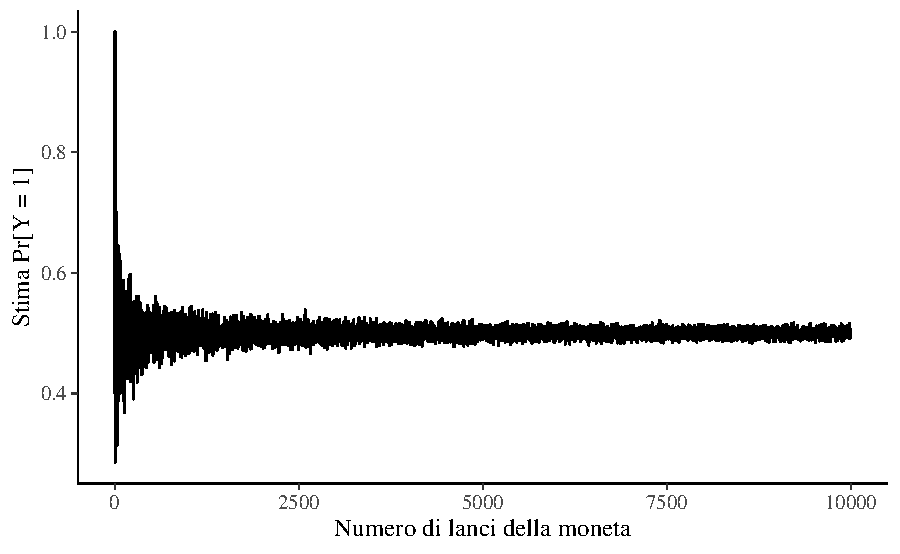
\includegraphics{015_prob_intro_files/figure-latex/legge-grandi-n-1-1} 

}

\caption{Stima della probabilità di successo in funzione del numero di lanci di una moneta.}\label{fig:legge-grandi-n-1}
\end{figure}

Dato che il grafico \ref{fig:legge-grandi-n-1} su una scala lineare non rivela chiaramente l'andamento della simulazione, utilizzeremo invece un grafico in cui sull'asse \(x\) è stata imposta una scala logaritmica. Con l'asse \(x\) su scala logaritmica, i valori tra 1 e 10 vengono tracciati all'incirca con la stessa ampiezza come nel caso dei valori tra 50 e 700, eccetera.

\begin{Shaded}
\begin{Highlighting}[]
\NormalTok{d }\SpecialCharTok{\%\textgreater{}\%}
  \FunctionTok{ggplot}\NormalTok{(}
    \FunctionTok{aes}\NormalTok{(}\AttributeTok{x =}\NormalTok{ n, }\AttributeTok{y =}\NormalTok{ estimate)}
\NormalTok{  ) }\SpecialCharTok{+}
  \FunctionTok{geom\_line}\NormalTok{() }\SpecialCharTok{+}
  \FunctionTok{scale\_x\_log10}\NormalTok{(}
    \AttributeTok{breaks =} \FunctionTok{c}\NormalTok{(}
      \DecValTok{1}\NormalTok{, }\DecValTok{3}\NormalTok{, }\DecValTok{10}\NormalTok{, }\DecValTok{50}\NormalTok{, }\DecValTok{200}\NormalTok{,}
      \DecValTok{700}\NormalTok{, }\DecValTok{2500}\NormalTok{, }\DecValTok{10000}
\NormalTok{    )}
\NormalTok{  ) }\SpecialCharTok{+}
  \FunctionTok{theme}\NormalTok{(}\AttributeTok{legend.title =} \FunctionTok{element\_blank}\NormalTok{()) }\SpecialCharTok{+}
  \FunctionTok{labs}\NormalTok{(}
    \AttributeTok{x =} \StringTok{"Numero di lanci della moneta"}\NormalTok{,}
    \AttributeTok{y =} \StringTok{"Stima Pr[Y = 1]"}
\NormalTok{  )}
\end{Highlighting}
\end{Shaded}

\begin{figure}

{\centering 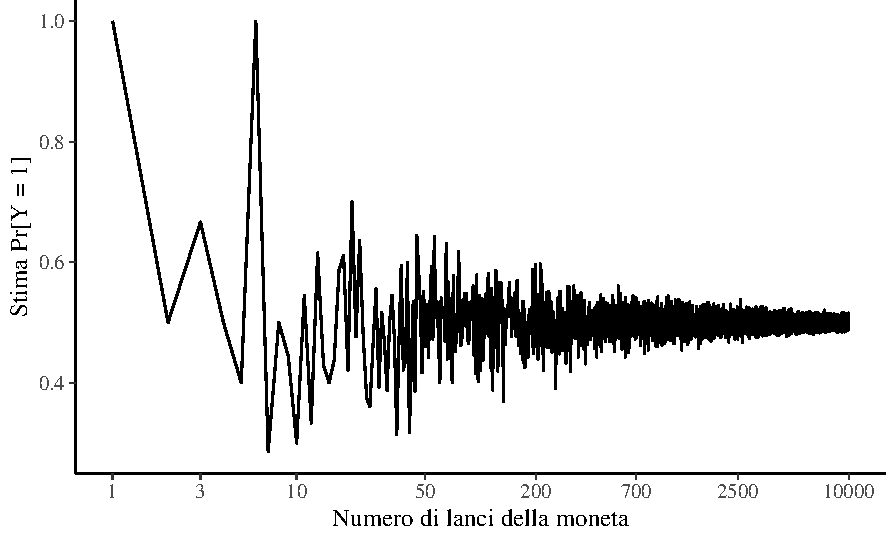
\includegraphics{015_prob_intro_files/figure-latex/legge-grandi-n-2-1} 

}

\caption{Stima della probabilità di successo in funzione del numero di lanci di una moneta -- scala logaritmica.}\label{fig:legge-grandi-n-2}
\end{figure}

La \emph{legge dei grandi numeri} ci dice che all'aumentare del numero di ripetizioni dell'esperimento casuale la media dei risultati ottenuti tenderà ad avvicinarsi al valore atteso man mano che verranno eseguite più prove. Nel caso presente, la figura \ref{fig:legge-grandi-n-2} mostra appunto che, all'aumentare del numero \emph{M} di lanci della moneta, la stima di \(Pr[Y = 1]\) tende a convergere al vero valore di 0.5.

\hypertarget{variabili-casuali-multiple}{%
\section{Variabili casuali multiple}\label{variabili-casuali-multiple}}

Le variabili casuali non esistono isolatamente. Abbiamo iniziato con una singola variabile casuale \emph{Y} che rappresenta il risultato di un singolo, specifico lancio di una moneta equlibrata. Ma supponiamo ora di lanciare la moneta tre volte. Ciò suggerisce che possiamo avere le variabili casuali \(Y_1 , Y_2 , Y_3\) che rappresentano i risultati di ciascuno dei lanci. Possiamo assumere che ogni lancio sia indipendente, ovvero che non dipenda dal risultato degli altri lanci. Ognuna di queste variabili \(Y_n\) per \(n \in 1:3\) ha \(Pr[Y_n =1]=0.5\) e \(Pr[Y_n =0]=0.5\).
Possiamo combinare più variabili casuali usando le operazioni aritmetiche. Se \(Y_1 , Y_2, Y_3\) sono variabili casuali che rappresentano tre lanci di una moneta equilibrata (o un lancio di tre monete equilibrate), possiamo definire la somma di tali variabili casuali come

\[
Z = Y_1 + Y_2 + Y_3.
\]

\noindent
Possiamo simulare i valori assunti dalla variabile casuale \emph{Z} simulando i valori di \(Y_1, Y_2, Y_3\) per poi sommarli.

\begin{Shaded}
\begin{Highlighting}[]
\NormalTok{y1 }\OtherTok{\textless{}{-}} \FunctionTok{rbinom}\NormalTok{(}\DecValTok{1}\NormalTok{, }\DecValTok{1}\NormalTok{, }\FloatTok{0.5}\NormalTok{)}
\NormalTok{y2 }\OtherTok{\textless{}{-}} \FunctionTok{rbinom}\NormalTok{(}\DecValTok{1}\NormalTok{, }\DecValTok{1}\NormalTok{, }\FloatTok{0.5}\NormalTok{)}
\NormalTok{y3 }\OtherTok{\textless{}{-}} \FunctionTok{rbinom}\NormalTok{(}\DecValTok{1}\NormalTok{, }\DecValTok{1}\NormalTok{, }\FloatTok{0.5}\NormalTok{)}
\FunctionTok{c}\NormalTok{(y1, y2, y3)}
\CommentTok{\#\textgreater{} [1] 0 0 0}
\NormalTok{z }\OtherTok{\textless{}{-}} \FunctionTok{sum}\NormalTok{(}\FunctionTok{c}\NormalTok{(y1, y2, y3))}
\FunctionTok{cat}\NormalTok{(}\StringTok{"z ="}\NormalTok{, z, }\StringTok{"}\SpecialCharTok{\textbackslash{}n}\StringTok{"}\NormalTok{)}
\CommentTok{\#\textgreater{} z = 0}
\end{Highlighting}
\end{Shaded}

\noindent
ovvero,

\begin{Shaded}
\begin{Highlighting}[]
\NormalTok{y }\OtherTok{\textless{}{-}} \FunctionTok{rep}\NormalTok{(}\ConstantTok{NA}\NormalTok{, }\DecValTok{3}\NormalTok{)}
\ControlFlowTok{for}\NormalTok{ (i }\ControlFlowTok{in} \DecValTok{1}\SpecialCharTok{:}\DecValTok{3}\NormalTok{) \{}
\NormalTok{  y[i] }\OtherTok{\textless{}{-}} \FunctionTok{rbinom}\NormalTok{(}\DecValTok{1}\NormalTok{, }\DecValTok{1}\NormalTok{, }\FloatTok{0.5}\NormalTok{)}
\NormalTok{\}}
\NormalTok{y}
\CommentTok{\#\textgreater{} [1] 1 1 0}
\NormalTok{z }\OtherTok{\textless{}{-}} \FunctionTok{sum}\NormalTok{(y)}
\FunctionTok{cat}\NormalTok{(}\StringTok{"z ="}\NormalTok{, z, }\StringTok{"}\SpecialCharTok{\textbackslash{}n}\StringTok{"}\NormalTok{)}
\CommentTok{\#\textgreater{} z = 2}
\end{Highlighting}
\end{Shaded}

\noindent
oppure, ancora più semplicemente:

\begin{Shaded}
\begin{Highlighting}[]
\NormalTok{y }\OtherTok{\textless{}{-}} \FunctionTok{rbinom}\NormalTok{(}\DecValTok{3}\NormalTok{, }\DecValTok{1}\NormalTok{, }\FloatTok{0.5}\NormalTok{)}
\NormalTok{y}
\CommentTok{\#\textgreater{} [1] 1 0 1}
\NormalTok{z }\OtherTok{\textless{}{-}} \FunctionTok{sum}\NormalTok{(y)}
\FunctionTok{cat}\NormalTok{(}\StringTok{"z ="}\NormalTok{, z, }\StringTok{"}\SpecialCharTok{\textbackslash{}n}\StringTok{"}\NormalTok{)}
\CommentTok{\#\textgreater{} z = 2}
\end{Highlighting}
\end{Shaded}

Possiamo ripetere questa simulazione \(M = 1e5\) volte:

\begin{Shaded}
\begin{Highlighting}[]
\NormalTok{M }\OtherTok{\textless{}{-}} \FloatTok{1e5}
\NormalTok{z }\OtherTok{\textless{}{-}} \FunctionTok{rep}\NormalTok{(}\ConstantTok{NA}\NormalTok{, M)}
\ControlFlowTok{for}\NormalTok{ (i }\ControlFlowTok{in} \DecValTok{1}\SpecialCharTok{:}\NormalTok{M) \{}
\NormalTok{  y }\OtherTok{\textless{}{-}} \FunctionTok{rbinom}\NormalTok{(}\DecValTok{3}\NormalTok{, }\DecValTok{1}\NormalTok{, }\FloatTok{0.5}\NormalTok{)}
\NormalTok{  z[i] }\OtherTok{\textless{}{-}} \FunctionTok{sum}\NormalTok{(y)}
\NormalTok{\}}
\end{Highlighting}
\end{Shaded}

\noindent
e calcolare una stima della probabilità che la variabile casuale \(Z\) assuma i valori 0, 1, 2, 3:

\begin{Shaded}
\begin{Highlighting}[]
\FunctionTok{table}\NormalTok{(z) }\SpecialCharTok{/}\NormalTok{ M}
\CommentTok{\#\textgreater{} z}
\CommentTok{\#\textgreater{}       0       1       2       3 }
\CommentTok{\#\textgreater{} 0.12608 0.37225 0.37666 0.12501}
\end{Highlighting}
\end{Shaded}

Nel caso di 4 monete equilibrate, avremo:

\begin{Shaded}
\begin{Highlighting}[]
\NormalTok{M }\OtherTok{\textless{}{-}} \FloatTok{1e5}
\NormalTok{z }\OtherTok{\textless{}{-}} \FunctionTok{rep}\NormalTok{(}\ConstantTok{NA}\NormalTok{, M)}
\ControlFlowTok{for}\NormalTok{ (i }\ControlFlowTok{in} \DecValTok{1}\SpecialCharTok{:}\NormalTok{M) \{}
\NormalTok{  y }\OtherTok{\textless{}{-}} \FunctionTok{rbinom}\NormalTok{(}\DecValTok{4}\NormalTok{, }\DecValTok{1}\NormalTok{, }\FloatTok{0.5}\NormalTok{)}
\NormalTok{  z[i] }\OtherTok{\textless{}{-}} \FunctionTok{sum}\NormalTok{(y)}
\NormalTok{\}}
\FunctionTok{table}\NormalTok{(z) }\SpecialCharTok{/}\NormalTok{ M}
\CommentTok{\#\textgreater{} z}
\CommentTok{\#\textgreater{}       0       1       2       3       4 }
\CommentTok{\#\textgreater{} 0.06303 0.24984 0.37314 0.25090 0.06309}
\end{Highlighting}
\end{Shaded}

Viene detta \emph{variabile casuale discreta} una variabile casuale le cui modalità possono essere costituite solo da numeri interi:

\[
\mathbb{Z} = \dots, -2, -1, 0, 1, 2, \dots
\]

\hypertarget{funzione-di-massa-di-probabilituxe0}{%
\section{Funzione di massa di probabilità}\label{funzione-di-massa-di-probabilituxe0}}

È conveniente avere una funzione che associa ogni possibile valore di una variabile casuale alla sua probabilità. In generale, ciò è possibile se e solo se la variabile casuale è discreta, così com'è stata definita nel Paragrafo precedente.

Ad esempio, se consideriamo \(Z = Y_1 + \dots + Y_4\) come il numero di risultati ``testa'' in 4 lanci della moneta, allora possiamo definire la seguente funzione:

\[
\begin{array}{rclll}
p_Z(0) & = & 1/16 & & \mathrm{TTTT}
\\
p_Z(1) & = & 4/16 & & \mathrm{HTTT, THTT, TTHT, TTTH}
\\
p_Z(2) & = & 6/16 & & \mathrm{HHTT, HTHT, HTTH, THHT, THTH, TTTH}
\\
p_Z(3) & = & 4/16 & & \mathrm{HHHT, HHTH, HTHH, THHH}
\\
p_Z(4) & = & 1/16 & & \mathrm{HHHH}
\end{array}
\]

Il lancio di quattro monete può produrre sedici possibili risultati. Dato che i lanci sono indipendenti e le monete sono equilibrate, ogni possibile risultato è ugualmente probabile. Nella tabella in alto, le sequenze dei risultati possibili del lancio delle 4 monete sono riportate nella colonna più a destra. Le probabilità si ottengono dividendo il numero di sequenze che producono lo stesso numero di eventi testa per il numero dei risultati possibili.

La funzione \(p_Z\) è stata costruita per mappare un valore \(u\) per \(Z\) alla probabilità dell'evento \(Z = u\). Convenzionalmente, queste probabilità sono scritte come

\[
p_Z(z) = \mbox{Pr}[Z = z].
\]
\noindent
La parte a destra dell'uguale si può leggere come: ``la probabilità che la variabile casuale \(Z\) assuma il valore \(z\)''.

Una funzione definita come sopra è detta \emph{funzione di massa di probabilità} della variabile casuale \(Z\). Ad ogni variabile casuale discreta è associata un'unica funzione di massa di probabilità.

Una rappresentazione grafica della stima della funzione di massa di probabilità per l'esperimento casuale del lancio di quattro monete equilibrate è fornita nella figura \ref{fig:barplot-mdf-4coins}.

\begin{Shaded}
\begin{Highlighting}[]
\FunctionTok{set.seed}\NormalTok{(}\DecValTok{1234}\NormalTok{)}
\NormalTok{M }\OtherTok{\textless{}{-}} \FloatTok{1e5}
\NormalTok{nflips }\OtherTok{\textless{}{-}} \DecValTok{4}
\NormalTok{u }\OtherTok{\textless{}{-}} \FunctionTok{rbinom}\NormalTok{(M, nflips, }\FloatTok{0.5}\NormalTok{)}
\NormalTok{x }\OtherTok{\textless{}{-}} \DecValTok{0}\SpecialCharTok{:}\NormalTok{nflips}
\NormalTok{y }\OtherTok{\textless{}{-}} \FunctionTok{rep}\NormalTok{(}\ConstantTok{NA}\NormalTok{, nflips }\SpecialCharTok{+} \DecValTok{1}\NormalTok{)}
\ControlFlowTok{for}\NormalTok{ (n }\ControlFlowTok{in} \DecValTok{0}\SpecialCharTok{:}\NormalTok{nflips) \{}
\NormalTok{  y[n }\SpecialCharTok{+} \DecValTok{1}\NormalTok{] }\OtherTok{\textless{}{-}} \FunctionTok{sum}\NormalTok{(u }\SpecialCharTok{==}\NormalTok{ n) }\SpecialCharTok{/}\NormalTok{ M}
\NormalTok{\}}
\NormalTok{bar\_plot }\OtherTok{\textless{}{-}}
  \FunctionTok{data.frame}\NormalTok{(}\AttributeTok{Z =}\NormalTok{ x, }\AttributeTok{count =}\NormalTok{ y) }\SpecialCharTok{\%\textgreater{}\%}
  \FunctionTok{ggplot}\NormalTok{(}
    \FunctionTok{aes}\NormalTok{(}\AttributeTok{x =}\NormalTok{ Z, }\AttributeTok{y =}\NormalTok{ count)}
\NormalTok{  ) }\SpecialCharTok{+}
  \FunctionTok{geom\_bar}\NormalTok{(}\AttributeTok{stat =} \StringTok{"identity"}\NormalTok{) }\SpecialCharTok{+}
  \FunctionTok{scale\_x\_continuous}\NormalTok{(}
    \AttributeTok{breaks =} \DecValTok{0}\SpecialCharTok{:}\DecValTok{4}\NormalTok{,}
    \AttributeTok{labels =} \FunctionTok{c}\NormalTok{(}\DecValTok{0}\NormalTok{, }\DecValTok{1}\NormalTok{, }\DecValTok{2}\NormalTok{, }\DecValTok{3}\NormalTok{, }\DecValTok{4}\NormalTok{)}
\NormalTok{  ) }\SpecialCharTok{+}
  \FunctionTok{labs}\NormalTok{(}
    \AttributeTok{y =} \StringTok{"Probabilità stimata Pr[Z = z]"}
\NormalTok{  )}
\NormalTok{bar\_plot}
\end{Highlighting}
\end{Shaded}

\begin{figure}

{\centering 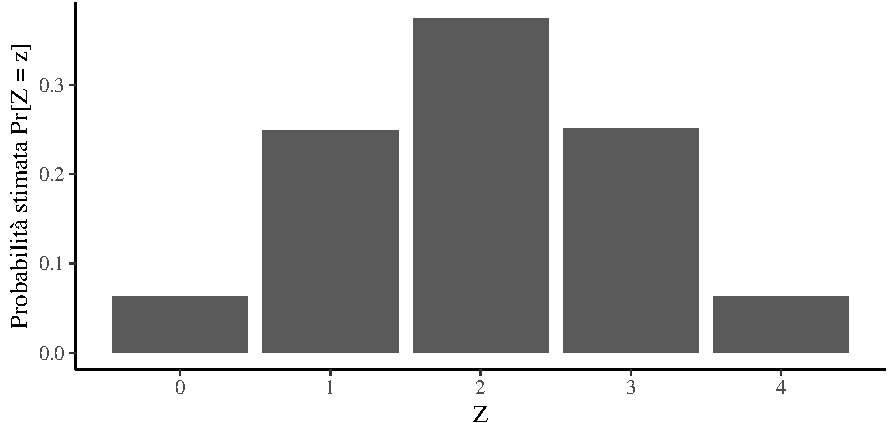
\includegraphics{015_prob_intro_files/figure-latex/barplot-mdf-4coins-1} 

}

\caption{Grafico di $M = 100\,000$ simulazioni della funzione di massa di probabilità di una variabile casuale definita come il numero di teste in quattro lanci di una moneta equilibrata.}\label{fig:barplot-mdf-4coins}
\end{figure}

Se \(A\) è un sottoinsieme della variabile casuale \(Z\), allora denotiamo
con \(P_{z}(A)\) la probabilità assegnata ad \(A\) dalla distribuzione
\(P_{z}\). Mediante una distribuzione di probabilità \(P_{z}\) è dunque
possibile determinare la probabilità di ciascun sottoinsieme
\(A \subset Z\) come

\[
P_{z}(A) = \sum_{z \in A} P_{z}(Z).
\]

\begin{example}
Per esempio, la probabilità che \(Z\) sia un numero dispari è

\[
Pr(\text{Z è un numero dispari}) = P_{z}(Z = 1) + P_{z}(Z = 3) = \frac{4}{16} + \frac{4}{16} = \frac{1}{2}.
\]
\end{example}

\hypertarget{considerazioni-conclusive}{%
\section*{Considerazioni conclusive}\label{considerazioni-conclusive}}
\addcontentsline{toc}{section}{Considerazioni conclusive}

In questo capitolo abbiamo visto come si costruisce lo spazio
campionario di un esperimento casuale, quali sono le proprietà di base
della probabilità e come si assegnano le probabilità agli eventi
definiti sopra uno spazio campionario discreto. Abbiamo anche introdotto
le nozioni di ``variabile casuale'', ovvero di una variabile che prende i suoi valori casualmente. E abbiamo descritto il modo di specificare la probabilità con cui sono presi i differenti valori, ovvero la funzione di distribuzione probabilistica

\[
F(X) = Pr(X < x),
\]
e la funzione di massa di probabilità. Le procedure di analisi dei dati psicologici che discuteremo in seguito faranno un grande uso di questi concetti e della notazione qui introdotta.

\hypertarget{part-inferenza-bayesiana}{%
\part*{Inferenza Bayesiana}\label{part-inferenza-bayesiana}}
\addcontentsline{toc}{part}{Inferenza Bayesiana}

\hypertarget{chapter-intro-bayes-inference}{%
\chapter{Il problema inverso}\label{chapter-intro-bayes-inference}}

La statistica descrittiva si occupa della descrizione, sintesi e presentazione delle informazioni contenute nei dati osservati. Essa spesso rappresenta la fase preliminare di uno studio e un ausilio per l'individuazione di possibili modelli da utilizzare nella successiva fase dell'analisi inferenziale. A differenza della statistica descrittiva, quella inferenziale assume che le osservazioni siano il risultato di un campionamento statistico e il suo obiettivo è ricavare informazioni circa l'intera popolazione a partire dall'osservazione di un suo sottoinsieme.

L'aleatorietà del campione è l'aspetto sostanziale che distingue la statistica inferenziale dalla statistica descrittiva. Nel caso più semplice, il campione statistico è trattato come un insieme di realizzazioni di una variabile casuale assunta a modello del fenomeno oggetto di indagine. La natura del campionamento statistico e la distribuzione di tale variabile casuale determinano il modello statistico. La statistica inferenziale consente di stimare, verificare ipotesi, o effettuare previsioni sul fenomeno in esame.

L'inferenza Bayesiana è un approccio all'inferenza statistica in cui le probabilità non sono interpretate come frequenze, proporzioni o concetti analoghi, ma piuttosto come il grado di fiducia che una singola persona attribuisce al verificarsi di un evento sulla base delle proprie conoscenze e delle informazioni di cui dispone.

Nell'approccio bayesiano non si fa riferimento ad un modello probabilistico \(f(y \mid \theta)\) rappresentativo del fenomeno d'interesse noto a meno del valore assunto dal parametro (o dei parametri) che lo caratterizza. Si fa invece riferimento ad una distribuzione congiunta (di massa o di densità di probabilità) \(f(y, \theta)\). Entrambi gli argomenti della funzione \(y\) e \(\theta\) hanno natura di variabili casuali, laddove la nostra incertezza relativa a \(y\) è dovuta alla naturale variabilità del fenomeno indagato (\emph{variabilità aleatoria}), mentre la nostra incertezza relativa a \(\theta\) è dovuta alla mancata conoscenza del suo valore numerico (\emph{variabilità epistemica}).

\hypertarget{inferenza-bayesiana-come-un-problema-inverso}{%
\section{Inferenza bayesiana come un problema inverso}\label{inferenza-bayesiana-come-un-problema-inverso}}

L'inferenza bayesiana è formulata nei termini di un problema inverso che segue la regola di Bayes (si veda la Sezione \ref{inf-stat-probl-inv}). Per fissare la notazione, nel seguito \(y\) rappresenterà le variabili osservate, ovvero i dati, e \(\theta\) rappresenterà i parametri incogniti di un modello statistico. Sia \(y\) che \(\theta\) sono concepiti come delle variabili casuali. Con \(x\) verranno invece denotate le quantità note, come i predittori nel modello di regressione.

\hypertarget{funzioni-di-probabilituxe0}{%
\subsection{Funzioni di probabilità}\label{funzioni-di-probabilituxe0}}

L'inferenza bayesiana utilizza le seguenti distribuzioni di probabilità (o densità di probabilità):

\begin{itemize}
\item
  la \emph{distribuzione a priori} \(p(\theta)\) --- la credenza iniziale riguardo alla credibilità di ciascun valore \(\theta\);
\item
  la \emph{funzione di verosimiglianza} \(p(y \mid \theta)\) --- la credibilità che il ricercatore assegnerebbe ai dati osservati se conoscesse il parametro di interesse \(\theta\);
\item
  la \emph{verosimiglianza marginale} \(p(y)\) --- quanto sono credibili i dati \(y\) alla luce della nostra credenza a priori relativamente a \(\theta\). In termini formali:
  \[
  p(y) = \int_\theta p(y, \theta) d\theta = \int_\theta p(y \mid \theta) p(\theta) d\theta.
  \]
\item
  la \emph{distribuzione a posteriori} \(p(\theta \mid y)\) --- la nuova credenza a posteriori relativamente alla credibilità di ciascun valore \(\theta\) alla luce dei dati \(Y = y\).
\end{itemize}

\hypertarget{la-regola-di-bayes}{%
\subsection{La regola di Bayes}\label{la-regola-di-bayes}}

Nel contesto di un modello statistico, la formula di Bayes permette di giungere alla distribuzione a posteriori \(p(\theta \mid y)\) per il parametro di interesse \(\theta\), come indicato dalla seguente catena di equazioni:
\begin{align}
p(\theta \mid y)  &= \displaystyle \frac{p(\theta,y)}{p(y)}
 \ \ \ \ \ \mbox{ [definizione di probabilità condizionata]}
\\
&= \displaystyle \frac{p(y \mid \theta) \, p(\theta)}{p(y)}
 \ \ \ \ \ \mbox{ [legge della probabilità composta]}
\\
&=  \displaystyle \frac{p(y \mid\theta) \, p(\theta)}
                        {\int_{\Theta} p(y,\theta) \, d\theta}
 \ \ \ \ \ \mbox{ [legge della probabilità totale]}
\\
&= \displaystyle \frac{p(y \mid\theta) \, p(\theta)}
                        {\int_{\Theta} p(y \mid\theta) \, p(\theta) \, d\theta}
 \ \ \ \ \ \mbox{ [legge della probabilità composta]}
\\
& \propto \displaystyle p(y \mid\theta) \, p(\theta)
\label{eq:bayesmodel}
\end{align}

La regola di Bayes ``inverte'' la probabilità della distribuzione a posteriori \(p(\theta \mid y)\), esprimendola nei termini della funzione di verosimiglianza \(p(y \mid \theta)\) e della distribuzione a priori \(p(\theta)\). L'ultimo passo è importante per la stima della distribuzione a posteriori mediante i metodi Monte Carlo a catena di Markov, in quanto per questi metodi richiedono soltanto che le funzioni di probabilità siano definite a meno di una costante di proporzionalità. In altri termini, per la maggior parte degli scopi dell'inferenza inversa, è sufficiente calcolare la densità a posteriori non normalizzata, ovvero è possibile ignorare il denominatore bayesiano \(p(y)\). La distribuzione a posteriori non normalizzata, dunque, si riduce al prodotto della varosimiglianza e della distribuzione a priori.

Possiamo dire che la regola di Bayes viene usata per aggiornare le credenze a priori su \(\theta\) (ovvero, la distribuzione a priori) in modo tale da produrre le nuove credenze a posteriori \(p(\theta \mid y)\) che combinano le informazioni fornite dai dati \(y\) con le credenze precedenti. La distribuzione a posteriori riflette dunque l'aggiornamento delle credenze del ricercatore alla luce dei dati.

La \eqref{eq:bayesmodel} rende evidente che, in ottica bayesiana, la quantità di interesse \(\theta\) non è fissata come nell'impostazione frequentista, ma è una variabile casuale la cui distribuzione di probabilità è influenzata sia dalle informazioni a priori sia dai dati a disposizione. In altre parole, nell'approccio bayesiano non esiste un valore vero di \(\theta\), ma vogliamo fornire invece un giudizio di probabilità. Prima delle osservazioni, sulla base delle nostre conoscenze assegniamo a \(\theta\) una distribuzione a priori di probabilità. Dopo le osservazioni, correggiamo il nostro giudizio e assegniamo a \(\theta\) una distribuzione a posteriori di probabilità. La distribuzione a posteriori \(p(\theta \mid y)\) contiene tutta l'informazione riguardante il parametro \(\theta\) e viene utilizzata per produrre indicatori sintetici, per la determinazione di stime puntuali o intervallari, e per la verifica d'ipotesi.

\hypertarget{inferenza-bayesiana}{%
\section{Inferenza bayesiana}\label{inferenza-bayesiana}}

Un esempio di inferenza bayesiana è quello nel quale i dati sono rappresentati da una proporzione. Per questo tipo di dati possiamo adottare il seguente modello statistico
\begin{equation}
y  \sim \mbox{Bin}(n, \theta),
\label{eq:binomialmodel}
\end{equation}
laddove \(\theta\) è la probabiltà che una prova Bernoulliana assuma il valore 1 e \(n\) corrisponde al numero di prove Bernoulliane. Questo modello assume che le prove Bernoulliane \(y_i\) che costituiscono il campione \(y\) siano tra loro indipendenti e che ciascuna abbia la stessa probabilità \(\theta \in [0, 1]\) di essere un ``successo'' (valore 1). In altre parole, il modello generatore dei dati avrà una funzione di massa di probabilità
\[
p(y \mid \theta)
\ = \
\mbox{Bin}(y \mid n, \theta).
\]

Nei capitoli precedenti è stato mostrato come, sulla base del modello binomiale, sia possibile assegnare una probabilità a ciascun possibile valore \(y \in \{0, 1, \dots, n\}\) \emph{assumendo noto il valore del parametro} \(\theta\). Ma ora abbiamo il problema inverso, ovvero quello di fare inferenza su \(\theta\) alla luce dei dati campionari \(y\). In altre parole, riteniamo di conoscere il modello probabilistico che ha generato i dati, ma di tale modello non conosciamo i parametri. Nel caso presente, il modello probabilistico è quello binomiale. Noi vogliamo ottenere informazioni sul valore di \(\theta\) conoscendo il numero \(y\) di successi osservati nel campione.

La \eqref{eq:binomialmodel} è un \emph{modello statistico}. Tale modello non spiega perché, in ciascuna realizzazione, \(Y\) assuma un particolare valore. Questo modello deve piuttosto essere inteso come un costrutto matematico che ha lo scopo di riflettere alcune proprietà del processo corrispondente ad una sequenza di prove Bernoulliane. In questo senso, è simile al modello di Isaac Newton dei moti planetari che utilizza equazioni differenziali. Le equazioni non sono i pianeti, ma solo descrizioni di come si muovono i pianeti in risposta alle forze gravitazionali. Modelli come quello di Newton ci permettono di prevedere alcuni fenomeni, come il moto dei pianeti, ad esempio. Ma in generale i modelli sono solo delle approssimazioni del fenomeno che vogliono descrivere. Anche il modello di Newton, che produce previsioni estremamente accurate di ciò che possiamo osservare a occhio nudo a proposito del moto dei corpi celesti, è solo un'approssimazione dei modelli del moto e dei fenomeni gravitazionali che, in seguito, sono stati introdotti da Albert Einstein. E anche tali modelli successivi sono, a loro volta, solo un caso speciale della più generale teoria della relatività. In altre parole, modelli sempre migliori vengono proposti, laddove ogni successivo modello è migliore di quello precedente in quanto ne migliora le capacità di previsione, è più generale, o è più elegante.

Una parte del lavoro della ricerca in tutte le scienze consiste nel verificare le assunzioni dei modelli e, se necessario, nel migliorare i modelli dei fenomeni considerati. Un modello viene giudicato in relazione al suo obiettivo. Se l'obiettivo del modello molto semplice che stiamo discutendo è quello di prevedere la proporzione di casi nei quali \(y_i = 1\), \(i = 1, \dots, n\), allora un modello con un solo parametro come quello che abbiamo introdotto sopra può essere sufficiente. Ma l'evento \(y_i=1\) (supponiamo: superare l'esame di Psicometria, oppure risultare positivi al COVID-19) dipende da molti fattori e se vogliamo rendere conto di una tale complessità, un modello come quello che stiamo discutendo qui certamente non sarà sufficiente.

Per concludere, un modello è un costrutto matematico il cui scopo è quello di rappresentare un qualche aspetto della realtà. Il valore di un tale strumento dipende dalla sua capacità di ottenere lo scopo per cui è stato costruito.

\hypertarget{notazione}{%
\subsection{Notazione}\label{notazione}}

Per rappresentare in un modo conciso i modelli statistici viene usata una notazione particolare. Ad esempio, invece di scrivere
\[
p(\theta) = \text{Beta}(1, 1),
\]
scriviamo:
\[
\theta \sim \text{Beta}(1, 1).
\]
Il simbolo ``\(\sim\)'' viene spesso letto ``è distribuito come''. Possiamo anche pensare che significhi che \(\theta\) costituisce un campione casuale estratto dalla distribuzione Beta(1, 1). Allo stesso modo, per l'esempio presente, la verosimiglianza può essere scritta come:
\[
y \sim \text{Bin}(n, \theta).
\]

\hypertarget{il-problema-inverso}{%
\subsection{Il problema inverso}\label{il-problema-inverso}}

Nel modello statistico che stiamo esaminando, il termine \(n\) viene trattato come una costante nota e \(\theta\) come una \emph{variabile casuale}. Il parametro \(\theta\) del modello rappresenta la probabilità che ciascuna prova Bernoulliana sia un ``successo''. Dato che \(\theta\) è incognito, ma abbiamo a disposione un campione di dati, l'inferenza su \(\theta\) può essere svolta, mediante la regola di Bayes, costruendo la distribuzione a posteriori \(p(\theta \mid y)\). Una volta ottenuta la distribuzione a posteriori possiamo riassumerla, ad esempio, riportando l'intervallo centrale al 95\% della distribuzione di densità, ovvero
\[
\mbox{Pr}\left[ 0.025 \leq \theta \leq 0.975
                \ \Big| \
        Y = y
         \right].
\]

Se vogliamo sapere, per esempio, se la probabilità di \(y_i=1\) sia maggiore di 0.5, possiamo calcolare la probabilità dell'evento
\[
\mbox{Pr}\left[\theta > \frac{1}{2}
                \ \Bigg| \
        Y = y
         \right].
\]

\hypertarget{cosuxe8-un-parametro-del-modello}{%
\subsection{Cos'è un parametro del modello?}\label{cosuxe8-un-parametro-del-modello}}

Il parametro di un modello è un valore che influenza la credibilità dei dati. Ad esempio, il singolo parametro \(\theta\) del modello binomiale determina la forma della funzione di verosimiglianza binomiale. Ricordiamo che, per il modello binomiale, la funzione di verosimiglianza è:
\[
p(y \mid \theta, n) = \text{Bin}(y, n, \theta) = \binom{n}{y}\theta^y(1-\theta)^{n-y}.
\]

\hypertarget{la-distribuzione-a-priori-sui-parametri}{%
\subsection{La distribuzione a priori sui parametri}\label{la-distribuzione-a-priori-sui-parametri}}

Quando adottiamo un approccio bayesiano, i parametri non più delle costanti incognite ma delle variabili casuali governate da una propria legge di distribuzione delle probabilità (probabilità a priori). La distribuzione a priori sui valori dei parametri \(p(\theta)\) è parte integrante del modello statistico. Ciò implica che due modelli bayesiani possono condividere la stessa funzione di verosimiglianza, ma tuttavia devono essere considerati come modelli diversi se specificano diverse distribuzioni a priori. Ciò significa che, quando diciamo ``Modello binomiale'', intendiamo in realtà un'intera classe di modelli, ovvero tutti i possibili modelli che hanno la stessa verosimiglianza ma diverse distribuzioni a priori su \(\theta\).

Nell'analisi dei dati bayesiana, la distribuzione a priori \(p(\theta)\) codifica le credenze del ricercatore a proposito dei valori dei parametri, prima di avere osservato i dati. Idealmente, le credenze a priori che supportano la specificazione di una distribuzione a priori dovrebbero essere supportate da una qualche motivazione, come ad esempio i risultati di ricerche precedenti, o altre motivazioni giustificabili.

\begin{itemize}
\tightlist
\item
  Quando una nuova osservazione (p.~es., vedo un cigno bianco) corrisponde alle mie convinzioni precedenti (p.~es., la maggior parte dei cigni sono bianchi) sto rafforzando le mie convinzioni precedenti: più nuove osservazioni (p.~es., più cigni bianchi vedo), più forti diventano le mie credenze precedenti.
\item
  Tuttavia, quando una nuova osservazione (p.~es., vedo un cigno nero) non corrisponde alle mie convinzioni precedenti, ciò contribuisca a diminuire la certezza delle mie convinzioni precedenti: più nuove osservazioni non corrispondenti raccolgo (p.~es., più cigni neri vedo ), più deboli diventano le mie convinzioni precedenti. Fondamentalmente, più forti sono le mie credenze precedenti, più osservazioni non corrispondenti (ad esempio, cigni neri) devo raccogliere per cambiarle.
\end{itemize}

Pertanto, da una prospettiva bayesiana, l'incertezza intorno ai parametri di un modello \emph{dopo} aver visto i dati (ovvero le distribuzioni a posteriori) deve includere anche le credenze precedenti. Se questo modo di ragionare sembra molto intuitivo, non è una coincidenza: vi sono infatti diverse teorie psicologiche che prendono l'aggiornamento bayesiano come modello di funzionamento di diversi processi cognitivi.

Oltre alla motivazione che giustifica una distribuzione a priori, possiamo distinguere tra diverse distribuzioni a priori in base a quanto fortemente impegnano il ricercatore a ritenere come plausibile un particolare intervallo di valori dei parametri. Il caso più estremo è quello che rivela una totale assenza di conoscenze a priori, il che conduce alle \emph{distribuzioni a priori non informative}, ovvero quelle che assegnano lo stesso livello di credibilità a tutti i valori dei parametri. Le distribuzioni a priori informative, d'altra parte, possono essere \emph{debolmente informative} o \emph{fortemente informative}, a seconda della forza della credenza che esprimono. Il caso più estremo di credenza a priori è quello che riassume il punto di vista del ricercatore nei termini di un \emph{unico valore} del parametro, il che assegna tutta la probabilità (massa o densità) su di un singolo valore di un parametro. Poiché questa non è più una distribuzione di probabilità, sebbene ne soddisfi la definizione, in questo caso si parla di una \emph{distribuzione a priori degenerata}.

La figura seguente mostra esempi di distribuzioni a priori non informative, debolmente o fortemente informative, così come una distribuzione a priori espressa nei termini di un valore puntuale per il modello Binomiale. Le distribuzione a priori illustrate di seguito sono le seguenti:

\begin{itemize}
\tightlist
\item
  \emph{non informativa} : \(\theta_c \sim \text{Beta}(1,1)\);
\item
  \emph{debolmente informativa} : \(\theta_c \sim \text{Beta}(5,2)\);
\item
  \emph{fortemente informativa} : \(\theta_c \sim \text{Beta}(50,20)\);
\item
  \emph{valore puntuale} : \(\theta_c \sim \text{Beta}(\alpha, \beta)\) con \(\alpha, \beta \rightarrow \infty\) e \(\frac{\alpha}{\beta} = \frac{5}{2}\).
\end{itemize}

\begin{figure}

{\centering 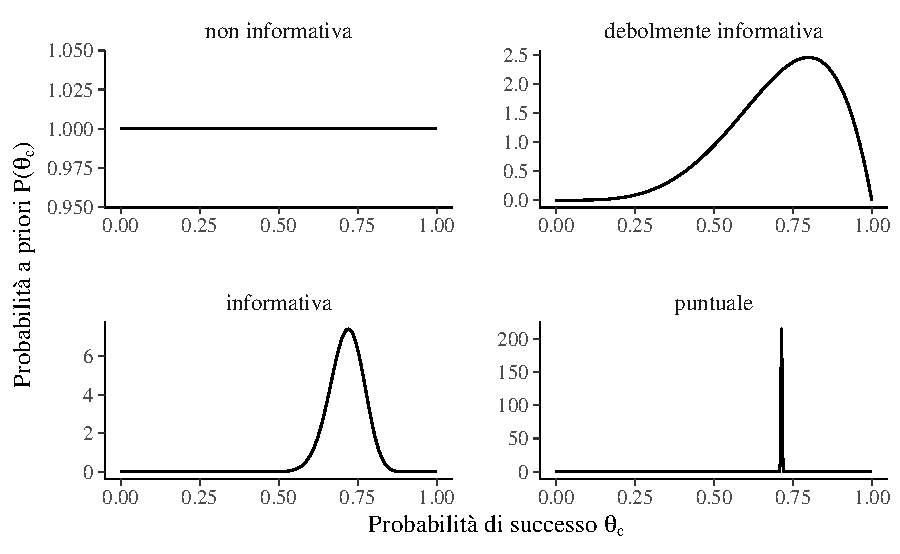
\includegraphics{025_intro_bayes_files/figure-latex/ch-03-02-models-types-of-priors-1} 

}

\caption{Esempi di distribuzioni a priori per il parametro $\theta_c$ nel Modello Binomiale.}\label{fig:ch-03-02-models-types-of-priors}
\end{figure}

\hypertarget{scelta-della-distribuzione-a-priori}{%
\subsection{Scelta della distribuzione a priori}\label{scelta-della-distribuzione-a-priori}}

La selezione delle distribuzioni a priori è stata spesso vista come una delle scelte più importanti che un ricercatore fa quando implementa un modello bayesiano in quanto può avere un impatto sostanziale sui risultati finali. La soggettività delle distribuzioni a priori è evidenziata dai critici come un potenziale svantaggio dei metodi bayesiani. A questa critica, \textcite{vandeSchoot2021modelling} rispondono dicendo che, al di là della scelta delle distribuzioni a priori, ci sono molti elementi del processo di inferenza statistica che sono soggettivi, ovvero la scelta del modello statistico e le ipotesi sulla distribuzione degli errori. In secondo luogo, \textcite{vandeSchoot2021modelling} notano come le distribuzioni a priori svolgono due importanti ruoli statistici: quello della ``regolarizzazione della stima'', ovvero, il processo che porta ad indebolire l'influenza indebita di osservazioni estreme, e quello del miglioramento dell'efficienza della stima, ovvero, la facilitazione dei processi di calcolo numerico di stima della distribuzione a posteriori. L'effetto della distribuzione a priori sulla distribuzione a posteriori verrà discusso nel Capitolo \ref{chapter-balance}.

\hypertarget{verosim-marginale}{%
\section{Verosimiglianza marginale}\label{verosim-marginale}}

Al denominatore della regola di Bayes abbiamo la verosimiglianza marginale \(p(y)\). Tale denominatore è espresso nei termini di un integrale che, tranne in pochi casi particolari, non ha una soluzione analitica.

\hypertarget{la-distribuzione-a-posteriori}{%
\section{La distribuzione a posteriori}\label{la-distribuzione-a-posteriori}}

Ci sono due metodi principali per calcolare la distribuzione a posteriori \(p(\theta \mid y)\):

\begin{itemize}
\tightlist
\item
  una precisa derivazione matematica formulata nei termini della distribuzione a priori coniugata alla distribuzione a posteriori (si veda il Capitolo \ref{chapter-distr-coniugate}); tale procedura però ha un'applicabilità molto limitata;
\item
  un metodo approssimato, molto facile da utilizzare in pratica, che dipende da metodi Monte Carlo basati su Catena di Markov (MCMC).
\end{itemize}

Una volta calcolata la distribuzione a posteriori dobbiamo riassumerla in qualche modo. Questo problema verrà discusso nel Capitolo \ref{chapter-sintesi-distr-post}.

\hypertarget{considerazioni-conclusive-1}{%
\section*{Considerazioni conclusive}\label{considerazioni-conclusive-1}}
\addcontentsline{toc}{section}{Considerazioni conclusive}

In base all'approccio bayesiano, invece di dire che il parametro di interesse di un modello statistico ha un valore vero ma sconosciuto, diciamo che, prima di eseguire l'esperimento, è possibile assegnare una distribuzione di probabilità, che chiamano stato di credenza, a quello che è il vero valore del parametro. Questa distribuzione a priori può essere nota (per esempio, sappiamo che la distribuzione dei punteggi del QI è normale con media 100 e deviazione standard 15) o può essere del tutto arbitraria. L'inferenza bayesiana procede poi nel modo seguente: si raccolgono alcuni dati e si calcola la probabilità dei possibili valori del parametro alla luce dei dati osservati e delle credenze a priori. Questa nuova distribuzione di probabilità è chiamata ``distribuzione a posteriori'' e riassume l'incertezza dell'inferenza.


% Bibliography
%%%%%%%%%%%%%%%%%%%%%%%%%%%%%%%%%%%%%%%%%%%%%%%%%%%%%%%%%%

\backmatter
\SmallMargins

\printbibliography
\onecolumn


% Tables (of tables, of figures)
%%%%%%%%%%%%%%%%%%%%%%%%%%%%%%%%%%%%%%%%%%%%%%%%%%%%%%%%%%


\cleardoublepage
\LargeMargins
\listoffigures


% After-body (LaTeX code inclusion)
%%%%%%%%%%%%%%%%%%%%%%%%%%%%%%%%%%%%%%%%%%%%%%%%%%%%%%%%%%




% Back cover
%%%%%%%%%%%%%%%%%%%%%%%%%%%%%%%%%%%%%%%%%%%%%%%%%%%%%%%%%%%

% Even page, small margins, no running head, no page number.
\evenpage
\SmallMargins
\thispagestyle{empty}

\begin{normalsize}

\begin{description}

\selectlanguage{italian}
\item[Abstract]
This document contains the material of the lessons of Psicometria B000286 (2021/2022) aimed at students of the first year of the Degree Course in Psychological Sciences and Techniques of the University of Florence, Italy.
\item[Keywords]
Data science, Bayesian statistics.
~\\

\end{description}

\end{normalsize}


\end{document}
